\Opensolutionfile{ans}[ans/CD20/Muc_7_8]
\setcounter{ex}{0}
\setcounter{dang}{0}
\section{Mức độ 7,8 điểm}
\begin{dang}
	{Bất phương trình logarit}
\end{dang}
\begin{ex}%{Tex 32 chuyên đề]%[Nhật Thiện]%[2D2B6-2]
	[Chuyên Vĩnh Phúc 2019]%Câu 1.
	Tập nghiệm của bất phương trình $2\log_2(x-1)\leq\log_2(5-x)+1$ là
	\choice
	{$[3; 5]$}
	{\True $(1; 3]$}
	{$[1; 3]$}
	{$(1; 5)$}
	\loigiai{
		Điều kiện $1<x<5$.\\
		Ta có
		\begin{eqnarray*}
			& &2\log_2(x-1)\leq\log_2(5-x)+1\Leftrightarrow\log_2(x-1)^2\leq\log_2[2(5-x)]\\
			&\Leftrightarrow&(x-1)^2\leq 10-2x\\
			&\Leftrightarrow& x^2-9\leq 0\Leftrightarrow-3\leq x\leq 3 
		\end{eqnarray*}
		Vậy tập nghiệm của bất phương trình là $S=(1;3]$.
	}
\end{ex}
\begin{ex}%{Tex 32 chuyên đề]%[Nhật Thiện]%[2D2B6-1]
	[THPT Gia Lộc Hải Dương 2019]%Câu 2.
	Tìm tập nghiệm $S$ của bất phương trình $2\log_3(4x-3)\leq\log_3(18x+27)$. 
	\choice
	{$S=\left[-\dfrac{3}{8}; 3\right]$}
	{\True $S=\left(\dfrac{3}{4}; 3\right]$}
	{$S=\left(\dfrac{3}{4};+\infty\right)$}
	{$S=[3;+\infty)$}
	\loigiai{
		$2\log_3(4x-3)\leq\log_3(18x+27)(*)$.\\
		Điều kiện $\heva{&4x-3>0\\&18x+27>0}\Leftrightarrow x>\dfrac{3}{4}$. \\
		Với điều kiện trên, 
		\begin{eqnarray*}
			& &(*)\Leftrightarrow\log_3(4x-3)^2\leq\log_3(18x+27)\\
			&\Leftrightarrow& (4x-3)^2\leq 18x+27\\
			&\Leftrightarrow& -\dfrac{3}{8}\leq x\leq 3.
		\end{eqnarray*}
		Kết hợp điều kiện ta được $S=\left(\dfrac{3}{4}; 3\right]$.
	}
\end{ex}
\begin{ex}%{Tex 32 chuyên đề]%[Nhật Thiện]%[2D2B6-3]
	[THPT Yên Khánh - Ninh Bình -2019]%Câu 3.
	Tập nghiệm của bất phương trình $\log_2^2(2x)+\log_2\dfrac{x}{4}<9$ chứa tập hợp nào sau đây?
	\choice
	{$\left(\dfrac{3}{2};6\right)$}
	{$(0;3)$}
	{$(1;5)$}
	{\True $\left(\dfrac{1}{2};2\right)$}
	\loigiai{
		Điều kiện $x>0$.\\
		Ta có
		\begin{eqnarray*}
			& &\log_2^2(2x)+\log_2\dfrac{x}{4}<9\Leftrightarrow(1+\log_2x)^2+\log_2x-2<9\\
			&\Leftrightarrow&\log_2^2x+3\log_2x-10<0\\
			&\Leftrightarrow&-5<\log_2x<2\Leftrightarrow\dfrac{1}{2^5}<x<4.
		\end{eqnarray*}
		Vậy $x\in\left(\dfrac{1}{2^5};4\right)$ chứa tập $\left(\dfrac{1}{2};2\right)$.
	}
\end{ex}
\begin{ex}%{Tex 32 chuyên đề]%[Nhật Thiện]%[2D2B6-2]
	[Chuyên Đại Học Vinh 2019]%Câu 4.
	Tập nghiệm của bất phương trình $\log_{\frac{1}{3}}(x-1)+\log_3(11-2x)\geq 0$ là 
	\choice
	{$(-\infty;4]$}
	{$(1;4]$}
	{$(1;4)$}
	{\True $\left[4;\dfrac{11}{2}\right)$}
	\loigiai{
		Điều kiện $\heva{&x-1>0\\&11-2x>0}\Leftrightarrow\heva{&x>1\\&x<\dfrac{11}{2}}\Leftrightarrow x\in\left(1;\dfrac{11}{2}\right)$.\\
		Ta có $\log_{\frac{1}{3}}(x-1)+\log_3(11-2x)\geq 0\Leftrightarrow\log_3\dfrac{11-2x}{x-1}\geq 0\Leftrightarrow\dfrac{11-2x}{x-1}\geq 0\Leftrightarrow x\in\left[1;\dfrac{11}{2}\right]$.\\
		Kết luận: $x\in\left(1;\dfrac{11}{2}\right)$. Vì $x\in\left[4;\dfrac{11}{2}\right)\subset\left(1;\dfrac{11}{2}\right)$.
	}
\end{ex}
\begin{ex}%{Tex 32 chuyên đề]%[Nhật Thiện]%[2D2B6-2]
	[Sở Phú Thọ 2019]%Câu 5.
	Tập nghiệm của bất phương trình $\log_{\frac{1}{3}}(x-1)+\log_3(11-2x)\geq 0$ là
	\choice
	{$(-\infty;4]$}
	{\True $(1;4]$}
	{$(1;4)$}
	{$\left[4;\dfrac{11}{2}\right)$}
	\loigiai{
		Điều kiện xác định: $1<x<\dfrac{11}{2}$.\\
		Khi đó ta có 
		\begin{eqnarray*}
			& &\log_{\frac{1}{3}}(x-1)+\log_3(11-2x)\geq 0\Leftrightarrow\log_3(11-2x)\geq\log_3(x-1)\Leftrightarrow 11-2x\geq x-1>0\\
			&\Leftrightarrow& \heva{&x>1\\&x\leq 4}\Leftrightarrow x\in(1;4] .
		\end{eqnarray*}
	}
\end{ex}
\begin{ex}%{Tex 32 chuyên đề]%[Nhật Thiện]%[2D2B6-2]
	[Sở Bắc Ninh 2019]%Câu 6.
	Tập nghiệm của bất phương trình $\log_{\frac{1}{3}}(x-1)+\log_3(11-2x)\geq 0$ là 
	\choice
	{$S=(-\infty; 4]$}
	{$S=(1; 4)$}
	{\True $S=(1; 4]$}
	{$S=\left(3;\dfrac{11}{2}\right)$}
	\loigiai{Ta có
		\begin{eqnarray*}
			& &\log_{\frac{1}{3}}(x-1)+\log_3(11-2x)\geq 0\Leftrightarrow\log_3(11-2x)-\log_3(x-1)\geq 0\\
			&\Leftrightarrow& \log_3(11-2x)\geq\log_3(x-1)\Leftrightarrow\heva{&11-2x\geq x-1\\&x-1>0}\Leftrightarrow 1<x\leq 4.
		\end{eqnarray*}
		Suy ra tập nghiệm của bất phương trình là $S=(1; 4]$.
	}
\end{ex}
\begin{ex}%{Tex 32 chuyên đề]%[Nhật Thiện]%[2D2B6-2]
	[THPT Nguyễn Khuyến 2019]%Câu 7.
	Tổng tất cả các nghiệm nguyên của bất phương trình $2\log_2\sqrt{x+1}\leq 2-\log_2(x-2)$ bằng
	\choice
	{$12$}
	{$9$}
	{$5$}
	{\True $3$}
	\loigiai{
		Điều kiện $\heva{&x+1>0\\&x-2>0}\Leftrightarrow\heva{&x >-1\\&x>2}\Leftrightarrow x>2$.\\
		Khi đó 
		\begin{eqnarray*}
			& &2\log_2\sqrt{x+1}\leq 2-\log_2(x-2)\Leftrightarrow\log_2(x+1)\leq\log_2\dfrac{4}{(x-2)}\Leftrightarrow x+1\leq\dfrac{4}{(x-2)}\\
			&\Leftrightarrow& \dfrac{x^2-x-2-4}{x-2}\leq 0\Leftrightarrow\dfrac{x^2-x-6}{x-2}\leq 0\Leftrightarrow x\in(-\infty;-2]\cup[2;3].
		\end{eqnarray*}
		Suy ra nghiệm của bất phương trình là $x\in(2;3]$.\\
		Nghiệm nguyên là $x=3$. Vậy tổng tất cả các nghiệm nguyên là $3$.
	}
\end{ex}
\begin{ex}%{Tex 32 chuyên đề]%[Nhật Thiện]%[2D2B6-3]
	[Mã 123 2017]%Câu 8.
	Tìm tập nghiệm $S$ của bất phương trình $\log_2^2x-5\log_2x+4\geq 0$. 
	\choice
	{$S=(-\infty;1]\cup [4;+\infty)$}
	{$S=[2;16]$}
	{\True $S=(0;2]\cup [16;+\infty)$}
	{$(-\infty;2]\cup [16;+\infty)$}
	\loigiai{
		Điều kiện $x>0$.\\
		Bpt $\Leftrightarrow\hoac{&\log_2x\geq 4\\&\log_2x\leq 1}\Leftrightarrow\hoac{&x\geq 16\\&x\leq 2.}$ \\
		Kết hợp điều kiện ta có $S=(0;2]\cup[16;+\infty)$.
	}
\end{ex}
\begin{ex}%{Tex 32 chuyên đề]%[Nhật Thiện]%[2D2B6-3]
	Tập nghiệm $S$ của bất phương trình $\log_2^2x-5\log_2x-6\leq 0$ là
	\choice
	{\True $S=\left[\dfrac{1}{2};64\right]$}
	{$S=\left(0;\dfrac{1}{2}\right]$}
	{$S=[64;+\infty)$}
	{$S=\left(0;\dfrac{1}{2}\right]\cup[64;+\infty)$}
	\loigiai{
		$\log_2^2x-5\log_2x-6\leq 0$.\qquad$(1)$\\
		Điều kiện $x>0(*)$.\\
		Đặt $t=\log_2x(2)$.\\
		$(1)$ thành $t^2-5t-6\leq 0\Leftrightarrow-1\leq t\leq 6\overset{(2)}{\Leftrightarrow}-1\leq\log_2x\leq 6\Leftrightarrow\dfrac{1}{2}\leq x\leq 64$.\\
		So với $(*)$: $(1)\Leftrightarrow\dfrac{1}{2}\leq x\leq 64$.\\
		Vậy $S=\left[\dfrac{1}{2};64\right]$.
	}
\end{ex}
\begin{ex}%{Tex 32 chuyên đề]%[Nhật Thiện]%[2D2K6-1]
	[Chuyên Vĩnh Phúc 2019]%Câu 10.
	Kí hiệu $\max\{a;b\}$ là số lớn nhất trong hai số $a,b$. Tìm tập nghiệm S của bất phương trình $\max\left\{\log_2x;\log_{\frac{1}{3}}x\right\}<1$. 
	\choice
	{\True $S=\left(\dfrac{1}{3};2\right)$}
	{$S=(0;2)$}
	{$S=\left(0;\dfrac{1}{3}\right)$}
	{$S=(2;+\infty)$}
	\loigiai{
		$y=\log_2x-\log_{\frac{1}{3}}x=\log_2x+\log_3x$.\\
		$y’=\dfrac{1}{x\ln 2}+\dfrac{1}{x\ln 3}>0,\forall x>0$ nên phương trình $y=0$ có nghiệm duy nhất.\\
		Mà phương trình $y=0$ có nghiệm $x=1$ do đó.\\
		Trường hợp 1: $x<1\colon\log_2x<\log_{\frac{1}{3}}x$.\\
		Ta có $\max\left\{\log_2x;\log_{\frac{1}{3}}x\right\}<1\cdot\Leftrightarrow\log_{\frac{1}{3}}x<1\Leftrightarrow x>\dfrac{1}{3}$.\\
		Do đó $\dfrac{1}{3}<x<1$.\\
		Trường hợp 2: $x\geq 1\colon\log_2x\geq\log_{\frac{1}{3}}x$.\\
		Ta có $\max\left\{\log_2x;\log_{\frac{1}{3}}x\right\}<1\cdot\Leftrightarrow\log_2x<1\Leftrightarrow x<2$.\\
		Do đó $1\leq x<2$.\\
		Vậy $S=\left(\dfrac{1}{3};2\right)$.\\
		$S=\left(\dfrac{1}{3};2\right)$.
	}
\end{ex}
\begin{ex}%{Tex 32 chuyên đề]%[Nhật Thiện]%[2D2K6-5]
	[Sở Bắc Ninh 2019]%Câu 11.
	Tập nghiệm của bất phương trình $\log_2\left(x\sqrt{x^2+2}+4-x^2\right)+2x+\sqrt{x^2+2}\leq 1$ là $\left(-\sqrt{a};-\sqrt{b}\right]$.\\
	Khi đó $a.b$ bằng
	\choice
	{$\dfrac{15}{16}$}
	{$\dfrac{12}{5}$}
	{\True $\dfrac{16}{15}$}
	{$\dfrac{5}{12}$}
	\loigiai{
		Ta có $x\sqrt{x^2+2}-x^2 =x\left(\sqrt{x^2+2}-x\right) =\dfrac{2x}{\sqrt{x^2+2}+x}$.\\
		Ta có 
		\begin{eqnarray*}
			& &\log_2\left(x\sqrt{x^2+2}+4-x^2\right)+2x+\sqrt{x^2+2}\leq 1\\
			&\Leftrightarrow&\log_2\left(x\left(\sqrt{x^2+2}-x\right)+4\right)+2x+\sqrt{x^2+2}\leq 1\\
			& \Leftrightarrow&\log_2\left(\dfrac{2x}{\sqrt{x^2+2}+x}+4\right)+2x+\sqrt{x^2+2}\leq 1\\
			&\Leftrightarrow& \log_2\dfrac{2\left(3x+2\sqrt{x^2+2}\right)}{\sqrt{x^2+2}+x}+2x+\sqrt{x^2+2}\leq 1.\qquad (1)
		\end{eqnarray*}
		Ta có $\sqrt{x^2+2}+x>0$, $\forall x\in\mathbb{R}$.\\
		Điều kiện $3x+2\sqrt{x^2+2}>0\Leftrightarrow 2\sqrt{x^2+2} >-3x\Leftrightarrow\hoac{&x\geq 0\\&\heva{&x<0\\&4x^2+8>9x^2}}\Leftrightarrow x >-\sqrt{\dfrac{8}{5}}$.\qquad$(*)$\\
		Với điều kiện $(*)$, ta có\\
		$(1)\Leftrightarrow\log_2\left(3x+2\sqrt{x^2+2}\right)+3x+2\sqrt{x^2+2}\leq\log_2\left(\sqrt{x^2+2}+x\right)+\sqrt{x^2+2}+x$.\qquad$(2)$\\
		Xét hàm số $f(t)=\log_2t+t$ với $t>0$. Có $f’(t)=\dfrac{1}{t\cdot\ln 2}+1>0$, $\forall t\in(0;+\infty)$.\\
		Hàm số $f(t)=\log_2t+t$ đồng biến trên $(0;+\infty),\left(3x+2\sqrt{x^2+2}\right)\in(0;+\infty)$ và $\left(\sqrt{x^2+2}+x\right)\in(0;+\infty)$.\\
		Nên 
		\begin{eqnarray*}
			(2)&\Leftrightarrow& f\left(3x+2\sqrt{x^2+2}\right)\leq f\left(\sqrt{x^2+2}+x\right)\\
			&\Leftrightarrow& 3x+2\sqrt{x^2+2}\leq\sqrt{x^2+2}+x\Leftrightarrow\sqrt{x^2+2}\leq-2x\Leftrightarrow\heva{&-2x\geq 0\\&x^2+2\leq 4x^2}\\
			&\Leftrightarrow&\heva{&x\leq 0\\&3x^2\geq 2}\Leftrightarrow x\leq-\sqrt{\dfrac{2}{3}}.
		\end{eqnarray*}
		Kết hợp với điều kiện ta có tập nghiệm bất phương trình là $\left(-\sqrt{\dfrac{8}{5}};-\sqrt{\dfrac{2}{3}}\right]$ hay $a\cdot b=\dfrac{16}{15}$.
	}
\end{ex}
\begin{ex}%{Tex 32 chuyên đề]%[Nhật Thiện]%[2D2K6-1]
	[Chuyên Đại học Vinh - 2019]%Câu 12.
	Bất phương trình $\left(x^3-9x\right)\ln(x+5)\leq 0$ có bao nhiêu nghiệm nguyên?
	\choice
	{$4$}
	{$7$}
	{\True $6$}
	{Vô số}
	\loigiai{
		Điều kiện $x >-5$.\\
		Cho $f(x)=\left(x^3-9x\right)\ln(x+5)=0\Leftrightarrow\hoac{&x^3-9x=0\\&\ln(x+5)=0}\Leftrightarrow\hoac{&x=-3\\&x=0\\&x=3\\&x=-4.}$ \\
		Bảng xét dấu
		\begin{center}
		\begin{tikzpicture}[scale=1, font=\footnotesize, line join=round, line cap=round, >=stealth]
			\tkzTabInit[nocadre=false,lgt=1.2,espcl=2.5,deltacl=0.6]
			{$x$ /0.6,$f(x)$ /0.6}
			{$-5$,$-4$,$-3$,$0$,$3$,$+\infty$}
			\tkzTabLine{,+,0,-,0,+,0,-,0,+,}
		\end{tikzpicture}
		\end{center}
		Dựa vào bảng xét dấu ta thấy $f(x)\leq 0\Leftrightarrow\hoac{&-4\leq x\leq-3\\&0\leq x\leq 3.}$ \\
		Vì $x\in\mathbb{Z}\Rightarrow x\in\left\{-4;-3; 0; 1; 2; 3\right\}$.\\
		Vậy có 6 giá trị nguyên của $x$ thỏa bài toán.
	}
\end{ex}
\begin{ex}%{Tex 32 chuyên đề]%[Nhật Thiện]%[2D2K6-5]
	[Chuyên Đại học Vinh - 2019]%Câu 13.
	Tính tổng tất cả các nghiệm nguyên của bất phương trình $\log_2\left(x^2+3\right)-\log_2x+x^2-4x+1\leq 0$. 
	\choice
	{$4$}
	{\True $6$}
	{$5$}
	{$3$}
	\loigiai{
		Điều kiện $x>0$.\\
		Ta có
		$$\log_2\left(x^2+3\right)-\log_2x+x^2-4x+1\leq 0\Leftrightarrow\log_2\left(x^2+3\right)+x^2+3\leq\log_24x+4x.\qquad(*)$$
		Xét hàm số $f(t)=\log_2t+t$ trên $\mathscr{D}=(0;+\infty)$. \\
		Ta có
		$f’(t)=\dfrac{1}{t\ln 2}+1>0$, $\forall t\in \mathscr{D}\Rightarrow$ hàm số $f$ đồng biến trên $D$.\\
		Suy ra $(*)\Leftrightarrow f\left(x^2+3\right)\leq f(4x)\Leftrightarrow x^2+3\leq 4x\Leftrightarrow 1\leq x\leq 3$.\\
		Vậy tập hợp các nghiệm nguyên của bất phương trình là $\{1; 2; 3\}$.\\
		Nhận xét: Với cách hỏi và đáp án của câu này ta chỉ cần mở MODE 7 của máy tính cầm tay, nhập vế trái của bất phương trình và cho biến chạy từ 1 đến 6 là tìm được đáp án ngay.
	}
\end{ex}
\begin{ex}%{Tex 32 chuyên đề]%[Nhật Thiện]%[2D2K6-5]
	[HKI - NK HCM - 2019]%Câu 14.
	Biết bất phương trình $\log_2\left(\dfrac{x^2+x+1}{16x+3}\right)+(\sqrt{x}-2)^2+x\leq 1$ có tập nghiệm là $S=(a;b)$. Hãy tính tổng $T=20a+10b$. 
	\choice
	{\True $T=45-10\sqrt{2}$}
	{$T=46-10\sqrt{2}$}
	{$T=46-11\sqrt{2}$}
	{$T=47-11\sqrt{2}$}
	\loigiai{
		Điều kiện $x\geq 0$.
		\begin{eqnarray*}
			& &\log_2\left(\dfrac{x^2+x+1}{16x+3}\right)+(\sqrt{x}-2)^2+x\leq 1\\
			&\Leftrightarrow&\log_2\left(x^2+x+1\right)-\log_2(16x+3)+2x-4\sqrt{x}+3\leq 0\\
			&\Leftrightarrow& \log_2\left(\left(x+\dfrac{1}{2}\right)^2+\dfrac{3}{4}\right)+2\left(\left(x+\dfrac{1}{2}\right)+\dfrac{3}{4}\right)\leq\log_2\left((2\sqrt{x})^2+\dfrac{3}{4}\right)+2\left(2\sqrt{x}+\dfrac{3}{4}\right) 
		\end{eqnarray*}
		Xét hàm số $f(t)=\log_2\left(t^2+\dfrac{3}{4}\right)+2\left(t+\dfrac{3}{4}\right)$ với $t\geq 0$ có $f’(t)=\dfrac{2t}{\left(t^2+\dfrac{3}{4}\right)\ln 2}+2>0$, $\forall t\geq 0$.\\
		nên $f(t)$ đồng biến trên khoảng $[0;+\infty)$.\\
		Suy ra 
		\begin{eqnarray*}
			& &\left(x+\dfrac{1}{2}\right)+\dfrac{3}{4}\leq 2\sqrt{x}+\dfrac{3}{4}\Leftrightarrow 2\sqrt{x}\geq x+\dfrac{1}{2}\\
			&\Leftrightarrow&\heva{&x\geq 0\\&x^2-3x+\dfrac{1}{4}\leq 0}\Leftrightarrow\dfrac{3-2\sqrt{2}}{2}\leq x\leq\dfrac{3+2\sqrt{2}}{2}\\
			&\Rightarrow& a=\dfrac{3-2\sqrt{2}}{2};b=\dfrac{3+2\sqrt{2}}{2}\Rightarrow T=20a+10b=45-10\sqrt{2} .
		\end{eqnarray*}
	}
\end{ex}
\begin{ex}%{Tex 32 chuyên đề]%[Nhật Thiện]%[2D2K6-1]
	[Chuyên Phan Bội Châu - Nghệ An - 2018]%Câu 15.
	Số nghiệm nguyên của bất phương trình $\log_2x+\log_3x\geq 1+\log_2x\cdot\log_3x$ là
	\choice
	{$1$}
	{\True $2$}
	{$3$}
	{Vô số}
	\loigiai{
		Điều kiện xác định: $x>0$.\\
		Ta có
		\begin{eqnarray*}
			& &\log_2x+\log_3x\geq 1+\log_2x\cdot\log_3x\Leftrightarrow(\log_2x-1)(\log_3x-1)\leq 0\\
			&\Leftrightarrow& \hoac{&\heva{&\log_2x-1\leq 0\\&\log_3x-1\geq 0}\\&\heva{&\log_2x-1\geq 0\\&\log_3x-1\leq 0}}\Leftrightarrow\hoac{&\heva{&0<x\leq 2\\&x\geq 3}\\&\heva{&x\geq 2\\&0<x\leq 3}}\Leftrightarrow 2\leq x\leq 3 
		\end{eqnarray*}
		Do đó có $2$ nghiệm nguyên thỏa mãn.
	}
\end{ex}
\begin{ex}%{Tex 32 chuyên đề]%[Nhật Thiện]%[2D2K6-1]
	[THPT Lý Thái Tổ - Bắc Ninh - 2018]%Câu 16.
	Bất phương trình $\log_2\left(\log_{\frac{1}{3}}\dfrac{3x-7}{x+3}\right)\geq 0$ có tập nghiệm là $(a; b]$. Tính giá trị $P=3a-b$. 
	\choice
	{$P=5$}
	{\True $P=4$}
	{$P=10$}
	{$P=7$}
	\loigiai{
		Ta có 
		\begin{eqnarray*}
			& &\log_2\left(\log_{\frac{1}{3}}\dfrac{3x-7}{x+3}\right)\geq 0\Leftrightarrow\heva{&\dfrac{3x-7}{x+3}>0\\&\log_{\frac{1}{3}}\dfrac{3x-7}{x+3}>0\\&\log_{\frac{1}{3}}\dfrac{3x-7}{x+3}\geq 1}\\
			&\Leftrightarrow&\heva{&\dfrac{3x-7}{x+3}>0\\&\dfrac{3x-7}{x+3}<1\\&\dfrac{3x-7}{x+3}\leq\dfrac{1}{3}}\Leftrightarrow\heva{&\dfrac{3x-7}{x+3}>0\\&\dfrac{3x-7}{x+3}\leq\dfrac{1}{3}}\\
			&\Leftrightarrow&\heva{&\dfrac{3x-7}{x+3}>0\\&\dfrac{8(x-3)}{3(x+3)}\leq 0}\Leftrightarrow\heva{&x\in(-\infty;-3)\cup\left(\dfrac{7}{3};+\infty\right)\\&\dfrac{8(x-3)}{3(x+3)}<0,\, x\in[-3; 3]}\Leftrightarrow x\in\left(\dfrac{7}{3}; 3\right].
		\end{eqnarray*}
		Suy ra $a=\dfrac{7}{3}$; $b=3$. Vậy $P=3a-b=3\cdot\dfrac{7}{3}-3=4$.
	}
\end{ex}
\begin{ex}%{Tex 32 chuyên đề]%[Nhật Thiện]%[2D2K6-1]
	[THPT Ngô Quyền - Hải Phòng - 2018]%Câu 17.
	Tập nghiệm của bất phương trình $\log_{\frac{1}{3}}(-\log_2x)<0$ là
	\choice
	{$(0; 5)$}
	{$(1; 2)$}
	{$\left(\dfrac{1}{4}; 4\right)$}
	{\True $\left(0;\dfrac{1}{2}\right)$}
	\loigiai{
		Điều kiện xác định: $\heva{&x>0\\&-\log_2x>0}\Leftrightarrow\heva{&x>0\\&x<1}\Rightarrow 0<x<1$.\\
		Ta có 
		$$\log_{\frac{1}{3}}(-\log_2x)<0\Leftrightarrow-\log_2x>1\Leftrightarrow\log_2x <-1\Leftrightarrow x<\dfrac{1}{2}.$$
		So sánh điều kiện, suy ra $S=\left(0;\dfrac{1}{2}\right)$.
	}
\end{ex}
\begin{ex}%{Tex 32 chuyên đề]%[Nhật Thiện]%[2D2B6-3]
	[THPT Nam Trực - Nam Định - 2018]%Câu 18.
	Tổng các nghiệm nguyên của bất phương trình $\log_{\sqrt{5}}^2x^5-25\log_{\sqrt{5}}x^2-75\leq 0$ là
	\choice
	{$70$}
	{$64$}
	{$62$}
	{\True $66$}
	\loigiai{
		Điều kiện $x>0$.\\
		Ta có 
		$$\log_{\sqrt{5}}^2x^5-25\log_{\sqrt{5}}x^2-75\leq 0\Leftrightarrow 4\log_5^2x-4\log_5x-3\leq 0\Leftrightarrow -\dfrac{1}{2}\leq\log_5x\leq\dfrac{3}{2}\Leftrightarrow\dfrac{1}{\sqrt{5}}\leq x\leq\sqrt{125}.$$ 
		Nghiệm nguyên của bất phương trình là $0;1;2;3;4;5;6;7;8;9;10;11$.\\
		$S=1+2+\cdots +11=\dfrac{11\cdot (11+1)}{2}=66$.
	}
\end{ex}
\begin{ex}%{Tex 32 chuyên đề]%[Nhật Thiện]%[2D2K6-1]
	[THPT Lương Văn Can - 2018]%Câu 19.
	Cho bất phương trình $(\log x+1)(4-\log x)>0$. Có bao nhiêu số nguyên $x$ thoả mãn bất phương trình trên. 
	\choice
	{$10000$}
	{$10001$}
	{$9998$}
	{\True $9999$}
	\loigiai{
		$(\log x+1)(4-\log x)>0(1)$.\\
		Điều kiện $x>0$.\\
		Khi ấy $(1)\Leftrightarrow-1<\log x<4\Leftrightarrow\dfrac{1}{10}<x<10000$. Vì $x\in\mathbb{Z}$ nên $x\in\left\{1;2;3;\ldots;9999\right\}$.\\
		Vậy có tất cả $9999$ số nguyên $x$ thoả mãn bất phương trình trên.
	}
\end{ex}
\begin{ex}%{Tex 32 chuyên đề]%[Nhật Thiện]%[2D2K6-5]
	[Chuyên Vinh – 2022]%Câu 20.
	Số nghiệm nguyên của bất phương trình $$\sqrt{2\log_2(x+2)}-\sqrt{\log_2\left(2x^2-1\right)}\geq (x+1)(x-5)$$ là
	\choice
	{$5$}
	{\True $6$}
	{$7$}
	{$4$}
	\loigiai{
		Nhận xét $x=-1$ là nghiệm của bất phương trình.\\
		Với $x\geq 1$ ta có
		\begin{eqnarray*}
			& &\sqrt{2\log_2(x+2)}-\sqrt{\log_2\left(2x^2-1\right)}\geq (x+1)(x-5)\\
			&\Leftrightarrow&\sqrt{\log_2\left(x^2+4x+4\right)}-\sqrt{\log_2\left(2x^2-1\right)}\geq x^2-4x-5.\qquad(2)
		\end{eqnarray*}
		Đặt $\heva{&a=2x^2-1\\&b=x^2+4x+4}$ $(a\geq 1;b\geq 1)$.\\
		Khi đó $(2) \Leftrightarrow b+\sqrt{\log_2b}\geq a+\sqrt{\log_2a}$.\qquad$(3)$\\
		Xét hàm số $f(t)=t+\sqrt{\log_2t}$ với $t\geq 1$.\\
		$f’(t)=1+\dfrac{1}{2t\sqrt{\log_2t}\ln 2}>0,\forall t>1$.\\
		Hàm số $f(t)$ đồng biến trên khoảng $(1;+\infty)$ nên từ $(3)$ ta có
		$$b\geq a\Leftrightarrow x^2+4x+4\geq 2x^2-1\Leftrightarrow-x^2+4x+5\geq 0\Leftrightarrow-1\leq x\leq 5.$$
		Mà $x\geq 1\Rightarrow 1\leq x\leq 5$.\\
		Vậy có $6$ giá trị nguyên của $x$ thỏa mãn.
	}
\end{ex}
\begin{ex}%{Tex 32 chuyên đề]%[Nhật Thiện]%[2D2K6-5]
	[Sở Hà Nam 2022]%Câu 21.
	Có bao nhiêu số nguyên $x$ thoả mãn $$\sqrt{2\log_3(x+2)}-\sqrt{\log_3\left(2x^2-1\right)}\geq(x+1)(x-5)?$$
	\choice
	{$8$}
	{\True $7$}
	{$6$}
	{$5$}
	\loigiai{
		Điều kiện xác định: $\heva{&x+2\geq 1\\&2x^2-1\geq 1}\Leftrightarrow\heva{&x\geq-1\\&x\leq-1\vee x\geq 1}\Leftrightarrow x\geq 1\Rightarrow D=[1;+\infty)$.\\
		Ta có 
		\begin{eqnarray*}
			& &\sqrt{2\log_3(x+2)}-\sqrt{\log_3\left(2x^2-1\right)}\geq(x+1)(x-5)\\
			&\Leftrightarrow& \sqrt{\log_3\left(x^2+4x+4\right)}+\left(x^2+4x+4\right)\geq\sqrt{\log_3\left(2x^2-1\right)}+\left(2x^2-1\right) .
		\end{eqnarray*}
		Đặt $f(t)=\sqrt{\log_3t}+t,\forall t\geq 1\Rightarrow f’(t)=\dfrac{1}{t\cdot\ln 3}\cdot\dfrac{1}{2\sqrt{\log_3t}}+1>0$, $\forall t>1$.\\
		Suy ra $f(t)$ đồng biến trên $(1;+\infty)$.\\
		Suy ra $f\left(x^2+4x+4\right)\geq f\left(2x^2-1\right)\Leftrightarrow x^2+4x+4\geq 2x^2-1\Leftrightarrow-1\leq x\leq 5$.\\
		Vậy có $7$ số nguyên $x$ thoả mãn.
	}
\end{ex}
\begin{dang}
	{Bất phương trình mũ}
\end{dang}
\begin{ex}%{Tex 32 chuyên đề]%[Nhật Thiện]%[2D2K6-3]
	[THPT Trần Phú - 2019]%Câu 1.
	Tập nghiệm của bất phương trình $\left(3^x+2\right)\left(4^{x+1}-8^{2x+1}\right)\leq 0$. 
	\choice
	{\True $\left[-\dfrac{1}{4};+\infty\right)$}
	{$\left(-\infty;-\dfrac{1}{4}\right]$}
	{$(-\infty;4]$}
	{$[4;+\infty)$}
	\loigiai{
		Ta có 
		\begin{eqnarray*}
			& &\left(3^x+2\right)\left(4^{x+1}-8^{2x+1}\right)\leq 0\Leftrightarrow 4^{x+1}-8^{2x+1}\leq 0\\
			&\Leftrightarrow& 4\cdot 2^{2x}-8\cdot\left(2^{2x}\right)^3\leq 0\Leftrightarrow-2\cdot\left(2^{2x}\right)^3+2^{2x}\leq 0.\qquad(*)
		\end{eqnarray*}
		Đặt $2^{2x}=t$, $t>0$, suy ra bất phương trình $(*)$ trở thành: $-2\cdot t^3+t\leq 0\Leftrightarrow\hoac{&-\dfrac{\sqrt{2}}{2}\leq t\leq 0\\&t\geq\dfrac{\sqrt{2}}{2}.}$ \\
		Giao với Đk $t>0$ ta được: $t\geq\dfrac{\sqrt{2}}{2}\Leftrightarrow 2^{2x}\geq\dfrac{\sqrt{2}}{2}\Leftrightarrow 2^{2x}\geq 2^{-\frac{1}{2}}\Leftrightarrow 2x\geq-\dfrac{1}{2}\Leftrightarrow x\geq-\dfrac{1}{4}$.\\
		Vậy tập nghiệm của BPT đã cho là $T=\left[-\dfrac{1}{4};+\infty\right)$.
	}
\end{ex}
\begin{ex}%{Tex 32 chuyên đề]%[Nhật Thiện]%[2D2B6-3]
	[Lý Nhân Tông - Bắc Ninh 2019]%Câu 2.
	Bất phương trình $3^{2x+1}-7\cdot 3^x+2>0$ có tập nghiệm là
	\choice
	{$(-\infty;-1)\cup\left(\log_23;+\infty\right)$}
	{$(-\infty;-2)\cup\left(\log_23;+\infty\right)$}
	{\True $(-\infty;-1)\cup\left(\log_32;+\infty\right)$}
	{$(-\infty;-2)\cup\left(\log_32;+\infty\right)$}
	\loigiai{
		Ta có $3^{2x+1}-7\cdot 3^x+2>0\Leftrightarrow 3\cdot (3^x)^2-7\cdot 3^x+2>0$.\\
		Đặt $3^x=t>0$ ta được $\heva{&t>0\\&3t^2-7t+2>0}\Leftrightarrow\hoac{&0<t<\dfrac{1}{3}\\&t>2.}$ \\
		Suy ra $\hoac{&0<3^x<\dfrac{1}{3}\\&3^x>2}\Leftrightarrow\hoac{&0<3^x<3^{-1}\\&3^x>3^{\log_32}}\Leftrightarrow\hoac{&x <-1\\&x>\log_32.}$ \\
		Vậy bất phương trình có tập nghiệm là $(-\infty;-1)\cup\left(\log_32;+\infty\right)$.
	}
\end{ex}
\begin{ex}%{Tex 32 chuyên đề]%[Nhật Thiện]%[2D2B6-3]
	[Chuyên ĐH Vinh - 2019]%Câu 3.
	Biết tập nghiệm của bất phương trình $2^x<3-\dfrac{2}{2^x}$ là $(a; b)$. Giá trị $a+b$ bằng
	\choice
	{$3$}
	{$2$}
	{$0$}
	{\True $1$}
	\loigiai{
		Ta có $2^x<3-\dfrac{2}{2^x}\Leftrightarrow(2^x)^2-3\cdot (2^x)+2<0\Leftrightarrow 1<2^x<2\Leftrightarrow 0<x<1$.\\
		Tập nghiệm của bất phương trình là $S=(0; 1)$.\\
		Suy ra $a=0$ và $b=1$ nên $a+b=1$.
	}
\end{ex}
\begin{ex}%{Tex 32 chuyên đề]%[Nhật Thiện]%[2D2K6-3]
	[Chuyên Bắc Giang 2019]%Câu 4.
	Tập nghiệm của bất phương trình $3^{3x+1}-9+3^{x+1}-9\cdot 3^{2x}>0$ là
	\choice
	{$(-\infty; 1)$}
	{$(3;+\infty)$}
	{\True $(1;+\infty)$}
	{$(-\infty; 3)$}
	\loigiai{
		Ta có $3^{3x+1}-9+3^{x+1}-9\cdot 3^{2x}>0\Leftrightarrow 3\cdot 3^{3x}-9+3\cdot 3^x-9\cdot 3^{2x}>0$.\\
		Đặt $3^x=t(t>0)$.\\
		Ta có bất phương trình 
		\begin{eqnarray*}
			& &3t^3-9+3t-9t^2>0\\
			&\Leftrightarrow& 3t^3-9t^2+3t-9>0\\
			&\Leftrightarrow& 3t^2(t-3)+3(t-3)>0\\
			&\Leftrightarrow& \left(3t^2+3\right)(t-3)>0\\
			&\Leftrightarrow& t-3>0\\&\Leftrightarrow t>3.
		\end{eqnarray*}
		Khi đó ta có $3^x>3\Leftrightarrow x>1$.\\
		Vậy tập nghiệm của bất phương trình là $S=(1;+\infty)$.
	}
\end{ex}
\begin{ex}%{Tex 32 chuyên đề]%[Nhật Thiện]%[2D2B6-3]
	[THPT Đông Sơn 1 - Thanh Hóa - 2019]%Câu 5.
	Bất phương trình $6.4^x-13\cdot 6^x+6\cdot 9^x>0$ có tập nghiệm là
	\choice
	{$S=(-\infty;-1)\cup[1;+\infty)$}
	{$S=(-\infty;-2)\cup(1;+\infty)$}
	{\True $S=(-\infty;-1)\cup(1;+\infty)$}
	{$S=(-\infty;-2]\cup[2;+\infty)$}
	\loigiai{
		Ta có $6.4^x-13\cdot 6^x+6\cdot 9^x>0\Leftrightarrow 6\cdot\left(\dfrac{2}{3}\right)^{2x}-13\cdot\left(\dfrac{2}{3}\right)^x+6>0\Leftrightarrow\hoac{&\left(\dfrac{2}{3}\right)^x>\dfrac{3}{2}\\&\left(\dfrac{2}{3}\right)^x<\dfrac{2}{3}}\Leftrightarrow\hoac{&x <-1\\&x>1.}$ \\
		Vậy tập nghiệm của bất phương trình là $S=(-\infty;-1)\cup(1;+\infty)$.
	}
\end{ex}
\begin{ex}%{Tex 32 chuyên đề]%[Nhật Thiện]%[2D2K6-2]
	[Kinh Môn - Hải Dương 2019]%Câu 6.
	Cho bất phương trình: $2.5^{x+2}+5\cdot 2^{x+2}-133\cdot\sqrt{10^x}\leq 0$ có tập nghiệm là $S=[a;b]$. Biểu thức $A=1000b-5a$ có giá trị bằng
	\choice
	{$2021$}
	{\True $2020$}
	{$2019$}
	{$2018$}
	\loigiai{
		Ta có 
		\begin{eqnarray*}
			& &2.5^{x+2}+5\cdot 2^{x+2}-133\cdot\sqrt{10^x}\leq 0\Leftrightarrow 50\cdot\left(5^{\frac{x}{2}}\right)^2-133\cdot 5^{\frac{x}{2}}\cdot 2^{\frac{x}{2}}+20\cdot\left(2^{\frac{x}{2}}\right)^2\leq 0\\
			&\Leftrightarrow& \left({2\cdot 5}^{\frac{x}{2}}-5\cdot 2^{\frac{x}{2}}\right)\left({25\cdot 5}^{\frac{x}{2}}-4\cdot 2^{\frac{x}{2}}\right)\leq 0\Leftrightarrow\left({2\cdot 5}^{\frac{x}{2}}-5\cdot 2^{\frac{x}{2}}\right)\left(5^{\frac{x}{2}+2}-2^{\frac{x}{2}+2}\right)\leq 0 \\
			&\Leftrightarrow& \hoac{&\heva{&{2\cdot 5}^{\frac{x}{2}}-5\cdot 2^{\frac{x}{2}}\leq 0\\&{25\cdot 5}^{\frac{x}{2}}-4\cdot 2^{\frac{x}{2}}\geq 0}\\&\heva{&{2\cdot 5}^{\frac{x}{2}}-5\cdot 2^{\frac{x}{2}}\geq 0\\&{25\cdot 5}^{\frac{x}{2}}-4\cdot 2^{\frac{x}{2}}\leq 0}}
			\Leftrightarrow \hoac{&\heva{&5^{\frac{x}{2}-1}\leq 2^{\frac{x}{2}-1}\\&5^{\frac{x}{2}+2}\geq 2^{\frac{x}{2}+2}}\\&\heva{&5^{\frac{x}{2}-1}\geq 2^{\frac{x}{2}-1}\\&5^{\frac{x}{2}+2}\leq 2^{\frac{x}{2}+2}}}\\
			&\Leftrightarrow& \hoac{&\heva{&\left(\dfrac{5}{2}\right)^{\frac{x}{2}-1}\leq 1\\&\left(\dfrac{5}{2}\right)^{\frac{x}{2}+2}\geq 1}\\&\heva{&\left(\dfrac{5}{2}\right)^{\frac{x}{2}-1}\geq 1\\&\left(\dfrac{5}{2}\right)^{\frac{x}{2}+2}\leq 1}}
			\Leftrightarrow\hoac{&\heva{&\dfrac{x}{2}-1\leq 0\\&\dfrac{x}{2}+2\geq 0}\\&\heva{&\dfrac{x}{2}-1\geq 0\\&\dfrac{x}{2}+2\leq 0}}\\
			&\Leftrightarrow&\hoac{&\heva{&x\leq 2\\&x\geq-4}\\&\heva{&x\geq 2\\&x\leq-4}} \\
			&\Leftrightarrow& -4\leq x\leq 2. 
		\end{eqnarray*}
	Suy ra $S=[-4;2]$. Vậy $A=1000b-5a=1000\cdot 2-5\cdot (-4)=2020$.
	}
\end{ex}
\begin{ex}%{Tex 32 chuyên đề]%[Nhật Thiện]%[2D2B6-2]
	[Toán Học Tuổi Trẻ Năm 2019]%Câu 7.
	Số nghiệm nguyên của bất phương trình: $\left(17-12\sqrt{2}\right)^x\geq(3+\sqrt{8})^{x^2}$ là 
	\choice
	{\True $3$}
	{$1$}
	{$2$}
	{$4$}
	\loigiai{
		Ta có
		\begin{eqnarray*}
			& &\left(17-12\sqrt{2}\right)^x\geq(3+\sqrt{8})^{x^2}\Leftrightarrow(3-\sqrt{8})^{2x}\geq(3+\sqrt{8})^{x^2}\\
			&\Leftrightarrow& (3+\sqrt{8})^{x^2+2x}\leq 1\Leftrightarrow x^2+2x\leq 0\Leftrightarrow x\in[-2;0].
		\end{eqnarray*}
		Vậy bất phương trình đã cho có $3$ nghiệm nguyên.
	}
\end{ex}
\begin{ex}%{Tex 32 chuyên đề]%[Nhật Thiện]%[2D2B6-4]
	[Chuyên Lê Quý Dôn Diện Biên 2019]%Câu 8.
	Tìm tập nghiệm của bất phương trình $2^x+2^{x+1}\leq 3^x+3^{x-1}$. 
	\choice
	{$(2;+\infty)$}
	{$(-\infty;2)$}
	{$(-\infty;2]$}
	{\True $[2;+\infty)$}
	\loigiai{
		Ta có 
		\begin{eqnarray*}
			& &2^x+2^{x+1}\leq 3^x+3^{x-1}\Leftrightarrow 3\cdot 2^x\leq 4\cdot 3^{x-1}\Leftrightarrow 2^{x-2}\leq 3^{x-2}\\
			&\Leftrightarrow& \left(\dfrac{2}{3}\right)^{x-2}\leq 1\Leftrightarrow x-2\geq 0\Leftrightarrow x\geq 2.
		\end{eqnarray*}
	}
\end{ex}
\begin{ex}%{Tex 32 chuyên đề]%[Nhật Thiện]%[2D2B6-3]
	[Chuyên Hưng Yên 2019]%Câu 9.
	Cho bất phương trình $\left(\dfrac{1}{3}\right)^{\frac{2}{x}}+3\left(\dfrac{1}{3}\right)^{\frac{1}{x}+1}>12$ có tập nghiệm $S=(a;b)$. Giá trị của biểu thức $P=3a+10b$ là
	\choice
	{$5$}
	{\True $-3$}
	{$-4$}
	{$2$}
	\loigiai{
		Đặt $t=\left(\dfrac{1}{3}\right)^{\frac{1}{x}} (t>0)$. Khi đó bất phương trình đã cho trở thành.\\
		$t^2+t>12\Leftrightarrow(t-3)(t+4)>0\Leftrightarrow t>3$ (vì $t>0$).\\
		Từ đó suy ra: $\left(\dfrac{1}{3}\right)^{\frac{1}{x}}>3\Leftrightarrow\dfrac{1}{x} <-1\Leftrightarrow-1<x<0$. Tập nghiệm của bất phương trình là $(-1;0)$.\\
		Vậy $a=-1$ và $b=0$. Suy ra $P=3a+10b=-3$.
	}
\end{ex}
\begin{ex}%{Tex 32 chuyên đề]%[Nhật Thiện]%[2D2B6-3]
	[Chuyên Hạ Long 2019]%Câu 10.
	Bất phương trình sau có bao nhiêu nghiệm nguyên dương $9^x-4\cdot 3^x+3<0$. 
	\choice
	{$3$}
	{$1$}     
	{\True $0$}
	{$2$}
	\loigiai{
		Đặt $t=3^x>0$.\\
		Bất phương trình đã cho trở thành $t^2-4\cdot t+3<0\Leftrightarrow 1<t<3\Leftrightarrow 1<3^x<3\Leftrightarrow 0<x<1$.\\
		Vậy bất phương trình đã cho có tập nghiệm là $S=(0,1)$ nên nó không có nghiệm nguyên dương.
	}
\end{ex}
\begin{ex}%{Tex 32 chuyên đề]%[Nhật Thiện]%[2D2B6-3]
	[THPT Đông Sơn Thanh Hóa 2019]%Câu 11.
	Bất phương trình $6.4^x-13\cdot 6^x+6\cdot 9^x>0$ có tập nghiệm là
	\choice
	{$S=(-\infty;-1)\cup[1;+\infty)$}
	{$S=(-\infty;-2)\cup(1;+\infty)$}
	{\True $S=(-\infty;-1)\cup(1;+\infty)$}
	{$S=(-\infty;-2]\cup[2;+\infty)$}
	\loigiai{
		Ta có $6.4^x-13\cdot 6^x+6\cdot 9^x>0\Leftrightarrow 6\cdot\left(\dfrac{2}{3}\right)^{2x}-13\cdot\left(\dfrac{2}{3}\right)^x+6>0\Leftrightarrow\hoac{&\left(\dfrac{2}{3}\right)^x>\dfrac{3}{2}\\&\left(\dfrac{2}{3}\right)^x<\dfrac{2}{3}}\Leftrightarrow\hoac{&x <-1\\&x>1.}$ \\
		Vậy tập nghiệm của bất phương trình là $S=(-\infty;-1)\cup(1;+\infty)$.
	}
\end{ex}
\begin{ex}%{Tex 32 chuyên đề]%[Nhật Thiện]
	[THPT Yên Khánh - Ninh Bình - 2019]%Câu 12.
	Tập nghiệm của bất phương trình $(2-\sqrt{3})^{x^2+4x-14}\geq 7+4\sqrt{3}$ là 
	\choice
	{\True $[-6;2]$}
	{$(-\infty-6]\cup[2;+\infty)$}
	{$(-6;2)$}
	{$(-\infty;-6)\cup(2;+\infty)$}
	\loigiai{
		Ta có 
		$7+4\sqrt{3}=(2+\sqrt{3})^2$, $(2-\sqrt{3})(2+\sqrt{3})=1$ và $2+\sqrt{3}=(2-\sqrt{3})^{-1}\Rightarrow 7+4\sqrt{3}=(2-\sqrt{3})^{-2}$.\\
		Khi đó
		\begin{eqnarray*}
			& &(2-\sqrt{3})^{x^2+4x-14}\geq 7+4\sqrt{3}\Leftrightarrow(2-\sqrt{3})^{x^2+4x-14}\geq(2-\sqrt{3})^{-2}\\
			&\Leftrightarrow& x^2+4x-14\leq-2\Leftrightarrow x^2+4x-12\leq 0\Leftrightarrow-6\leq x\leq 2.
		\end{eqnarray*}
		Vậy bất phương trình đã cho có tập nghiệm $[-6;2]$.
	}
\end{ex}
\begin{ex}%{Tex 32 chuyên đề]%[Nhật Thiện]%[2D2K6-1]
	[Chuyên Bắc Giang 2019]%Câu 13.
	Tìm số nghiệm nguyên của bất phương trình $6^x+4\leq 2^{x+1}+2\cdot 3^x$ 
	\choice
	{$2$}
	{$3$}
	{\True $1$}
	{$0$}
	\loigiai{
		Ta có 
		\begin{eqnarray*}
			& &6^x+4\leq 2^{x+1}+2\cdot 3^x\Leftrightarrow 6^x+4-2\cdot 2^x-2\cdot 3^x\leq 0\\
			&\Leftrightarrow& 2^x\left(3^x-2\right)+2\left(2-3^x\right)\leq 0 \\
			&\Leftrightarrow& \left(3^x-2\right)\left(2^x-2\right)\leq 0 \\
			&\Rightarrow& x\in[\log_32;1].
		\end{eqnarray*}
	}
\end{ex}
%%==========Câu 14
\begin{ex}%[2D2K6-5]
	[Chuyên Thái Bình 2019]%Câu 14.
	Tập nghiệm của bất phương trình $3^{x^2-9}+\left(x^2-9\right)\cdot 5^{x+1}<1$ là khoảng $(a; b)$. Tính $b-a$ 
	\choice
	{\True $6$}
	{$3$}
	{$8$}
	{$4$}
	\loigiai{
		$3^{x^2-9}+\left(x^2-9\right)\cdot 5^{x+1}<1 \quad(1)$. Ta có $5^{x+1}>0\,\forall x$.
		\begin{itemize}
			\item Xét $x^2-9=0$, VT $(1) =3^{\circ}+0=1$ (loại).
			\item Xét $x^2-9>0\Rightarrow\heva{&3^{x^2-9}>3^0=1\\&\left(x^2-9\right){\cdot 5}^{x+1}>0}\Rightarrow$ VT $(1) >1$ (loại).
			\item Xét $x^2-9<0\Rightarrow\heva{&3^{x^2-9}<3^0=1\\&\left(x^2-9\right){\cdot 5}^{x+1}<0}\Rightarrow$ VT $(1) <1$ luôn đúng.
		\end{itemize}
		Có $x^2-9<0\Leftrightarrow x\in(-3; 3)$.
		$ \Rightarrow $ Tập nghiệm của bất phương trình là $(-3; 3)\Rightarrow b-a=6$.}
\end{ex}
%%==========Câu 15
\begin{ex}%[2D2K6-3]
	[Hsg Bắc Ninh 2019]
	Bất phương trình $\dfrac{\sqrt{2+3^{2x}}}{\sqrt{2+3^{2x}}-\sqrt{2-3^{2x}}}+\dfrac{3^{4x}+\sqrt{4-3^{4x}}-7}{3^{2x}}\geq\dfrac{3^{2x}-2}{\sqrt{4-3^{4x}}-2+3^{2x}}$ có bao nhiêu nghiệm?
	\choice
	{Vô số}
	{\True $1$}
	{$2$}
	{$3$}
	\loigiai{
		Đặt $t=3^{2x}>0$, bất phương trình đã cho trở thành:\\ $\dfrac{\sqrt{2+t}}{\sqrt{2+t}-\sqrt{2-t}}+\dfrac{t^2+\sqrt{4-t^2}-7}{t}\geq\dfrac{t-2}{\sqrt{4-t^2}-2+t}\quad(1)$.\\
		Điều kiện: $0<t<2$.\\
		$(1)\Leftrightarrow\dfrac{\sqrt{2+t}\left(\sqrt{2+t}+\sqrt{2-t}\right)}{2t}+\dfrac{t^2+\sqrt{4-t^2}-7}{t}\geq\dfrac{t-2}{\sqrt{4-t^2}-2+t}$ \\
		$ \Leftrightarrow\dfrac{t+3\sqrt{4-t^2}+2t^2-12}{2t}\geq\dfrac{t-2}{\sqrt{4-t^2}-2+t}\Leftrightarrow\dfrac{t+3\sqrt{4-t^2}+2t^2-12}{2t}\geq\dfrac{(t-2)\left(\sqrt{4-t^2}+2-t\right)}{-2t^2+4t} $ \\
		$ \Leftrightarrow t+3\sqrt{4-t^2}+2t^2-12\geq-\sqrt{4-t^2}-2+t\Leftrightarrow 4\sqrt{4-t^2}+2t^2-10\geq 0 $ \\
		$ \Leftrightarrow\left(\sqrt{4-t^2}-1\right)^2\leq 0\Leftrightarrow t=\sqrt{3} $. Với $t=\sqrt{3}\Rightarrow 3^{2x}=\sqrt{3}\Leftrightarrow x=\dfrac{1}{4}$.\\
		Vậy bất phương trình có 1 nghiệm duy nhất.
	}
\end{ex}
%%==========Câu 16
\begin{ex}%[2D2K6-5]
	[KTNL GV Thpt Lý Thái Tổ 2019]%Câu 16.
	Số nghiệm nguyên thuộc đoạn $[-20; 20]$ của bất phương trình: $2^{2x+1}-9\cdot 2^x+4\sqrt{x^2+2x-3}\geq 0$ là
	\choice
	{$38$}
	{\True $36$}
	{$37$}
	{$19$}
	\loigiai{
		Điều kiện: $x^2+2x-3\geq 0\Leftrightarrow x\leq-3$ hoặc $x\geq 1$.\\
		Vì $x$ là số nguyên thuộc đoạn $[-20; 20]$ nên ta xét các trường hợp sau:
		\begin{itemize}
			\item $3\leq x\leq 20$, khi đó dễ thấy $2^{2x+1}-9\cdot 2^x=2^x\left(2^{x+1}-9\right)>0$ nên $2^{2x+1}-9\cdot 2^x+4\sqrt{x^2+2x-3}\geq 0$, do đó trên $[3; 20]$ bất phương trình có $18$ nghiệm nguyên.
			\item $x=2$ thay trực tiếp vào bất phương trình ta có: $4\sqrt{5}-4\geq 0$ (đúng). Do đó $x=2$ thỏa mãn yêu cầu bài toán.
			\item $x=1$ thay trực tiếp vào bất phương trình ta có: $-10\geq 0$ (sai). Do đó $x=1$ không thỏa mãn yêu cầu bài toán.
			\item $-20\leq x\leq-4$. Khi đó, xét hàm số: $f(x)=x^2+2x-3$, dễ thấy $\min\limits_{[-20;-4]} f(x)=f(-4)=5$ nên $4\sqrt{x^2+2x-3}\geq 4\sqrt{5},\forall x\in[-20;-4].\quad (a)$\\
			Mặt khác, đặt $t=2^x$, khi đó $2^{2x+1}-9\cdot 2^x=2t^2-9t$, $-20\leq x\leq-4\Rightarrow 2^{-20}\leq t\leq 2^{-4}$.\\
			Khi đó xét hàm số $g(t)=2t^2-9t$ với $2^{-20}\leq t\leq 2^{-4}$\\ 
			Dễ thấy $\min\limits_{\left[2^{-20}; 2^{-4}\right]} g(t)=g\left(2^{-4}\right)=-\dfrac{71}{128}.\quad (b)$\\
			Từ $(a),(b)$ suy ra $\min\limits_{[-20;-4]}\left\{h(x)=2^{2x+1}-9\cdot 2^x+4\sqrt{x^2+2x-3}\right\}=h(-4)=4\sqrt{5}-\dfrac{71}{128}>0$. Do đó bất phương trình đã cho nghiệm đúng với mọi $-20\leq x\leq-4$, nên trên đoạn $[-20;-4]$ bất phương trình có 17 nghiệm nguyên.
			\item Trường hợp $x=-3$ thay trực tiếp vào bất phương trình ta thấy không thỏa mãn.
		\end{itemize}
		Vậy số nghiệm nguyên của bất phương trình là 36.
	}
\end{ex}
%%==========Câu 17
\begin{ex}%[2D2K6-5]
	[Chuyên Thái Nguyên 2019]
	Tập hợp tất cả các số thực $x$ không thỏa mãn bất phương trình $9^{x^2-4}+\left(x^2-4\right)\cdot 2019^{x-2}\geq 1$ là khoảng $(a;b)$. Tính $b-a$. 
	\choice
	{$5$}
	{\True $4$}
	{$-5$}
	{$-1$}
	\loigiai{
		Xét hai trường hợp: $x^2-4\geq 0$ và $x^2-4<0$.
		\begin{itemize}
			\item $x^2-4\geq 0$. Khi đó ta có:
			$\heva{&9^{x^2-4}\geq 9^{\circ}=1\\&(x^2-4)\cdot{2019}^{x-2}\geq0}\Rightarrow 9^{x^2-4}+\left(x^2-4\right)2019^{x-2}\geq 1$.\\
			Dấu $=$ xảy ra $\Leftrightarrow x^2-4=0 \Leftrightarrow x=\pm 2$.
			\item $x^2-4<0\Leftrightarrow-2<x<2$. Khi đó ta có:\\
			$\heva{&9^{x^2-4}<9^{\circ}=1\\&(x^2-4)\cdot{2019}^{x-2}<0}\Rightarrow 9^{x^2-4}+\left(x^2-4\right)2019^{x-2}<1$ 
			$ \Rightarrow $ Bất phương trình vô nghiệm.
		\end{itemize}
		Vậy tập hợp tất cả các số thực x không thỏa mãn bất phương trình là
		$(-2;2)$.\\$\Rightarrow a=-2;b=2\Rightarrow b-a=4$.
	}
\end{ex}
%%==========Câu 18
\begin{ex}%[2D2K6-5]
	[Chuyên Bắc Ninh - 2020]
	Có bao nhiêu giá trị nguyên của $x$ trong đoạn $[0;2020]$ thỏa mãn bất phương trình sau $16^x+25^x+36^x\leq 20^x+24^x+30^x$. 
	\choice
	{$3$}
	{$2000$}
	{\True $1$}
	{$1000$}
	\loigiai{
		Ta có: $16^x+25^x+36^x\leq 20^x+24^x+30^x\Leftrightarrow 4^{2x}+5^{2x}+6^{2x}\leq 4^x\cdot 5^x+4^x\cdot 6^x+5^x\cdot 6^x$\\
		$\Leftrightarrow\left(4^x-5^x\right)^2+\left(4^x-6^x\right)^2+\left(5^x-6^x\right)^2\leq 0\Leftrightarrow\heva{&4^x-5^x=0\\&4^x-6^x=0\\&5^x-6^x=0}\Leftrightarrow\heva{&\left(\dfrac{4}{5}\right)^x=1\\&\left(\dfrac{4}{6}\right)^x=1\\&\left(\dfrac{5}{6}\right)^x=1}\Leftrightarrow x=0\in[0;2020]$.\\
		Vậy có 1 giá trị nguyên của $x$ trong đoạn $[0;2020]$ thỏa mãn bất phương trình.
	}
\end{ex}
%%==========Câu 19
\begin{ex}%[2D2K6-3]
	[Hải Hậu - Nam Định - 2020]
	Tập nghiệm của bất phương trình $(3^{2x}-9)(3^x-\dfrac{1}{27})\sqrt{3^{x+1}-1}\leq 0$ chứa bao nhiêu số nguyên?
	\choice
	{$2$}
	{\True $3$}
	{$4$}
	{$5$}
	\loigiai{
		Điều kiện $3^{x+1}-1\geq 0\Leftrightarrow 3^{x+1}\geq 1\Leftrightarrow x\geq-1$.\\
		Ta có $x=-1$ là một nghiệm của bất phương trình.\\
		Với $x >-1$, bất phương trình tương đương với $(3^{2x}-9)(3^x-\dfrac{1}{27})\leq 0$.\\
		Đặt $t=3^x>0$, ta có $(t^2-9)(t-\dfrac{1}{27})\leq 0\Leftrightarrow (t-3)(t+3)(t-\dfrac{1}{27})\leq 0\Leftrightarrow\hoac{&t\leq-3\\&\dfrac{1}{27}\leq t\leq 3}$.\\
		Kết hợp điều kiện $t=3^x>0$ ta được nghiệm $\dfrac{1}{27}\leq t\leq 3\Leftrightarrow\dfrac{1}{27}\leq 3^x\leq 3\Leftrightarrow-3\leq x\leq 1$.\\ Kết hợp điều kiện $x >-1$ ta được $-1<x\leq 1$ suy ra trường hợp này bất phương trình có 2 nghiệm nguyên.\\
		Vậy bất phương trình đã cho có tất cả 3 nghiệm nguyên.
	}
\end{ex}
%%==========Câu 20
\begin{ex}%[2D2K6-5]
	[THPT Lương Văn Tụy - Ninh Bình - 2018]
	Tập nghiệm của bất phương trình $9^x-2(x+5)\cdot 3^x+9(2x+1)\geq 0$ là
	\choice
	{\True $[0; 1]\cup[2;+\infty)$}
	{$(-\infty; 1]\cup[2;+\infty)$}
	{$[1; 2]$}
	{$(-\infty; 0]\cup[2;+\infty)$}
	\loigiai{
		Đặt $3^x=t$, $t>0$.\\
		Xét phương trình: $t^2-2(x+5)t+9(2x+1)=0.\quad (1)$\\
		Ta có $\Delta’=(x+5)^2-9(2x+1)=x^2-8x+16=(x-4)^2$ nên phương trình $(1)$ luôn có nghiệm.\\
		Nếu $x=4\Rightarrow\Delta’=0$ thì phương trình $(1)$ có nghiệm kép $t=x+5$.\\
		Do đó bất phương trình đã cho trở thành $3^x\geq x+5$ (luôn đúng khi $x=4$).\\
		Nếu $x\neq 4\Rightarrow\Delta’>0$ thì phương trình $(1)$ có hai nghiệm phân biệt $\hoac{&t=2x+1\\&t=9.}$ \\
		Xét các phương trình $3^x=9\Leftrightarrow x=2 \quad(1)$ và $3^x=2x+1\Leftrightarrow 3^x-2x-1=0. \quad(2)$\\
		Đặt $f(x)=3^x-2x-1$; ta có $f’(x)=3^x\ln 3-2$ là hàm số đồng biến trên $\mathbb{R}$.\\
		Lại có $f(0)=f(1)=0$ và $f’(0)<0$, $f’(1)>0$ nên $f’(x)$ đổi dấu một lần duy nhất trong $[0; 1]$.\\
		Vậy phương trình $(2)$ có đúng hai nghiệm $x=0$, $x=1$.\\
		Lập bảng xét dấu cho $(1)$ và $(2)$:\\
		\begin{tikzpicture}
			\tkzTabInit[deltacl=0.5,espcl=3,lgt=3]
			{$x$/1,$3^{x}-9$/1,$3^{x}-2x-1$/1,$VT$/1}
			{$-\infty$,$0$,$1$,$2$,$+\infty$}
			\tkzTabLine{,-,t,-,t,-,0,+}
			\tkzTabLine{,+,0,-,0,+,t,+}
			\tkzTabLine{,-,0,+,0,-,0,+}
		\end{tikzpicture}\\
		Tập nghiệm của bất phương trình là $S=[0; 1]\cup[2;+\infty)$.
	}
\end{ex}
%%==========Câu 21
\begin{ex}%[2D2K6-3]
	[Toán Học Tuổi Trẻ Số 6]
	Tập nghiệm của bất phương trình $2.7^{x+2}+7\cdot 2^{x+2}\leq 351\cdot\sqrt{14^x}$ có dạng là đoạn $S=[a;b]$. Giá trị $b-2a$ thuộc khoảng nào dưới đây?
	\choice
	{$\left(3;\sqrt{10}\right)$}
	{$(-4;2)$}
	{\True $\left(\sqrt{7};4\sqrt{10}\right)$}
	{$\left(\dfrac{2}{9};\dfrac{49}{5}\right)$}
	\loigiai{
		$2.7^{x+2}+7\cdot 2^{x+2}\leq 351\cdot\sqrt{14^x}\Leftrightarrow 49\cdot 7^x+28\cdot 2^x\leq 351\cdot\sqrt{14^x}\Leftrightarrow 49\cdot\sqrt{\dfrac{7^{2x}}{14^x}}+28\cdot\sqrt{\dfrac{2^{2x}}{14^x}}\leq 351$ \\
		$ \Leftrightarrow 49\cdot\sqrt{\dfrac{7^x}{2^x}}+28\cdot\sqrt{\dfrac{2^x}{7^x}}\leq 351 $. Đặt $t=\sqrt{\dfrac{7^x}{2^x}},t>0$ thì bpt trở thành $49t+\dfrac{28}{t}\leq 351$ \\
		$ \Leftrightarrow\dfrac{4}{49}\leq t\leq\dfrac{7}{2}\Rightarrow\dfrac{4}{49}\leq\sqrt{\dfrac{7^x}{2^x}}\leq\dfrac{7}{2}\Leftrightarrow-4\leq x\leq 2 $. Khi đó $S=[-4;2]$.\\
		Giá trị $b-2a=10\in\left(\sqrt{7};4\sqrt{10}\right)$.
	}
\end{ex}
%%==========Câu 22
\begin{ex}%[2D2K6-3]
	[Chuyên ĐHSPHN - 2018]
	Cho $f(x)=\dfrac{1}{2}\cdot 5^{2x+1}$; $g(x)=5^x+4x\cdot\ln 5$. Tập nghiệm của bất phương trình $f’(x)>g’(x)$ là
	\choice
	{$x<0$}
	{$x>1$}
	{$0<x<1$}
	{\True $x>0$}
	\loigiai{
		Ta có $f’(x)=\dfrac{1}{2}\cdot 5^{2x+1}\cdot (2x+1)’\cdot\ln 5=5^{2x+1}\cdot\ln 5$.\\
		Và: $g’(x)=5^x\cdot\ln 5+4\ln 5=\left(5^x+4\right)\ln 5$.\\
		Do đó: $f’(x)>g’(x)\Leftrightarrow 5^{2x+1}\cdot\ln 5>\left(5^x+4\right)\ln 5\Leftrightarrow 5^{2x+1}>5^x+4\Leftrightarrow 5\cdot 5^{2x}-5^x-4>0$ \\
		$ \Leftrightarrow\hoac{&5^x <-\dfrac{4}{5}(VN)\\&5^x>1}\Leftrightarrow 5^x>1\Leftrightarrow x>0 $.\\
		Vậy nghiệm của bất phương trình đã cho là $x>0$.
	}
\end{ex}
%%==========Câu 23
\begin{ex}%[2D2K6-3]
	[THPT Kinh Môn - Hải Dương - 2018]
	Bất phương trình $2.5^{x+2}+5\cdot 2^{x+2}\leq 133\cdot\sqrt{10^x}$ có tập nghiệm là $S=[a;b]$ thì biểu thức $A=1000b-4a+1$ có giá trị bằng
	\choice
	{$3992$}
	{$4008$}
	{$1004$}
	{\True $2017$}
	\loigiai{
		$2.5^{x+2}+5\cdot 2^{x+2}\leq 133\cdot\sqrt{10^x}\Leftrightarrow 50\cdot 5^x+20\cdot 2^x\leq 133\cdot\sqrt{10^x}\Leftrightarrow 50\cdot\left(\sqrt{\dfrac{5}{2}}\right)^x+20\cdot\left(\sqrt{\dfrac{2}{5}}\right)^x-133\leq 0$.\\
		Đặt $t=\left(\sqrt{\dfrac{5}{2}}\right)^x$, $t>0$, ta được bất phương trình: $50t^2-133t+20\leq 0\Leftrightarrow\dfrac{4}{25}\leq t\leq\dfrac{5}{2}$.\\
		Với $\dfrac{4}{25}\leq t\leq\dfrac{5}{2}$, ta có: $\dfrac{4}{25}\leq\left(\sqrt{\dfrac{5}{2}}\right)^x\leq\dfrac{5}{2}\Leftrightarrow-2\leq\dfrac{x}{2}\leq 1\Leftrightarrow-4\leq x\leq 2$.\\
		Tập nghiệm của bất phương trình là $S=[-4;2]\Rightarrow a=-4$, $b=2$. \\
		$ \Rightarrow A=1000b-4a+1 =1000\cdot 2-4(-4)+1 =2017 $.
	}
\end{ex}
%%==========Câu 24
\begin{ex}%[2D2K6-5]
	[Chuyên Biên Hòa - Hà Nam 2022]
	Tính tổng các nghiệm nguyên thuộc $[-5;10]$ của bất phương trình sau đây: $2^{x^2+x}\left(3x^2-6x+6\right)\geq 7x^2-29x+34$ 
	\choice
	{$54$}
	{$40$}
	{$55$}
	{\True $41$}
	\loigiai{
		Bất phương trình tương đương với: $2^{x^2+x-2}\left(12x^2-24x+24\right)\geq\left(7x^2-29x+34\right)$.\quad (1)\\
		Ta nhận thấy: $\left(12x^2-24x+24\right)-\left(7x^2-29x+34\right)=5x^2+5x-10=5\left(x^2+x-2\right)$ nên (1) trở thành:
		$2^{\frac{12x^2-24x+24}{5}}\left(12x^2-24x+24\right)\geq 2^{\frac{7x^2-29x+34}{5}}\left(7x^2-29x+34\right)$.\\
		Xét hàm số $y=f(t)=t\cdot 2^{\frac{t}{5}}$ có $f’(t)=2^{\frac{t}{5}}+\dfrac{t}{5}2^{\frac{t}{5}}\ln 2>0$ với mọi số thực $t$ nên suy ra hàm số $f(t)$ luôn đồng biến trên tức $12x^2-24x+24\geq 7x^2-29x+34\Leftrightarrow x^2+x-2\geq 0\Leftrightarrow\hoac{&x\geq 1\\&x\leq-2}.$ \\
		Mà $x\in [-5;10]$ nên $x\in [-5;-2]\cup [1;10]$. Suy ra tổng nghiệm nguyên của bất phương trình (1) là $S=\sum\limits_{k=-5}^{-2} X+\sum\limits_{k=1}^{10} X=41$.
	}
\end{ex}
\begin{dang}
	{Bất phương trình kết hợp mũ - logarit}
\end{dang}       
%%==========Câu 1
\begin{ex}%[2D2K6-5]
	[Mã 101 - 2021 Lần 1]
	Có bao nhiêu số nguyên $x$ thảo mãn $\left(3^{x^2}-9^x\right)\left[\log_3(x+25)-3\right]\leq 0$?
	\choice
	{$24$}
	{Vô số}
	{\True $26$}
	{$25$}
	\loigiai{
		Điều kiện: $x+25>0\Leftrightarrow x >-25$.\\
		Ta giải các phương trình:\\
		$3^{x^2}=9^x\Leftrightarrow x^2=2x\Leftrightarrow\hoac{&x=0\\&x=2}.$ \\
		$\log_3(x+25)=3\Leftrightarrow x+25=27\Leftrightarrow x=2$.\\
		Ta có bảng xét dấu sau:\\
		\begin{tikzpicture}
			\tkzTabInit[deltacl=0.5,espcl=3,lgt=3]
			{$x$/1,$3^{x^{2}}-9^{x}$/1,$\log_3(x+25)-3$/1,$VT$/1}
			{$-25$,$0$,$2$,$+\infty$}
			\tkzTabLine{,+,0,-,0,+}
			\tkzTabLine{,-,t,-,0,+}
			\tkzTabLine{,-,0,+,z,+}
		\end{tikzpicture}\\
		Dựa vào bảng xét dấu, để $\left(3^{x^2}-9^x\right)\left[\log_3(x+25)-3\right]\leq 0$ thì ta có\\
		$\hoac{&-25<x\leq 0\\&x=2}\xrightarrow{{x\in\mathbb{Z}}}\hoac{&-24\leq x\leq 0\\&x=2}$ có 26 giá trị nguyên của $x$ thỏa mãn.\\
	}
\end{ex}
%%==========Câu 2
\begin{ex}%[2D2K6-5]
	[Mã 102 - 2021 Lần 1]
	Có bao nhiêu số nguyên $x$ thỏa mãn $\left(3^{x^2}-9^x\right)\left[\log_2(x+30)-5\right]\leq 0$?
	\choice
	{$30$}
	{Vô số}
	{\True $31$}
	{$29$}
	\loigiai{
		Xét hàm số: $f(x)=\left(3^{x^2}-9^x\right)\left[\log_2(x+30)-5\right]$, với $x >-30$.\\
		Cho: $f(x)=0\Leftrightarrow\hoac{&3^{x^2}-9^x=0\\&\log_2(x+30)-5=0}\Leftrightarrow\hoac{&3^{x^2}=3^{2x}\\&x+30=2^5}\Leftrightarrow\hoac{&x=0\\&x=2}.$ \\
		Ta có bảng xét dấu như sau:\\
		\begin{tikzpicture}
			\tkzTabInit[deltacl=0.5,espcl=3,lgt=3]
			{$x$/1,$3^{x^{2}}-9^{x}$/1,$\log_2(x+30)-5$/1,$f(x)$/1}
			{$-30$,$0$,$2$,$+\infty$}
			\tkzTabLine{,+,0,-,0,+}
			\tkzTabLine{,-,t,-,0,+}
			\tkzTabLine{,-,0,+,0,+}
		\end{tikzpicture}\\
		Suy ra $f(x)\leq 0\Leftrightarrow\hoac{&-30<x\leq 0\\&x=2}.$ \\
		Mặt khác $x\in\mathbb{Z}$ nên $x\in\left\{-29;-28;-27;\ldots\cdots;-2;-1;0;2\right\}$.\\
		Vậy có $31$ số nguyên $x$ thỏa mãn.
	}
\end{ex}
%%==========Câu 3
\begin{ex}%[2D2K6-5]
	[Mã 104 - 2021 Lần 1]
	Có bao nhiêu số nguyên $x$ thỏa mãn $\left(2^{x^2}-4^x\right)\left[\log_3(x+25)-3\right]\leq 0$?
	\choice
	{$24$}
	{Vô số}
	{$25$}
	{\True $26$}
	\loigiai{
		Điều kiện: $x >-25$.\\
		Xét $2^{x^2}-4^x=0\Leftrightarrow x^2-2x=0\Leftrightarrow\hoac{&x=0\\&x=2}.$ \\
		Xét $\log_3(x+25)=3\Leftrightarrow x+25=27\Leftrightarrow x=2$.\\
		Ta có bảng xét dấu: \\
		\begin{tikzpicture}
			\tkzTabInit[deltacl=0.5,espcl=3,lgt=3]
			{$x$/1,$2^{x^{2}}-4^{x}$/1,$\log_3(x+25)-3$/1,$VT$/1}
			{$-25$,$0$,$2$,$+\infty$}
			\tkzTabLine{,+,0,-,0,+}
			\tkzTabLine{,-,t,-,0,+}
			\tkzTabLine{,-,0,+,0,+}
		\end{tikzpicture}\\
		Dựa vào bảng xét dấu ta có: BPT $\Leftrightarrow\hoac{&-25<x\leq 0\\&x=2}.$ \\
		Vì $x$ nguyên nên có 26 giá trị thỏa mãn bài toán.
	}
\end{ex}
%%==========Câu 4
\begin{ex}%[2D2K6-5]
	[Mã 103 - 2021 - Lần 1]
	Có bao nhiêu số nguyên $x$ thỏa mãn $\left(2^{x^2}-4^x\right)\left[\log_2(x+14)-4\right]\leq 0$?
	\choice
	{$14$}
	{$13$}
	{Vô số}
	{\True $15$}
	\loigiai{
		Điều kiện: $x >-14$.\\
		Bất phương trình tương đương: $\left(2^{x^2}-2^{2x}\right)\left[\log_2(x+14)-4\right]\leq 0$ \\
		$ \Leftrightarrow\hoac{&\heva{&2^{x^2}-2^{2x}\geq 0\\&\log_2(x+14)-4\leq 0}\\&\heva{&2^{x^2}-2^{2x}\leq 0\\&\log_2(x+14)-4\geq 0}}\Leftrightarrow\hoac{&\heva{&2^{x^2}\geq 2^{2x}\\&\log_2(x+14)\leq 4}\\&\heva{&2^{x^2}\leq 2^{2x}\\&\log_2(x+14)\geq 4}}\Leftrightarrow\hoac{&\heva{&x^2\geq 2x\\&x+14\leq 16}\\&\heva{&x^2\leq 2x\\&x+14\geq 16}}\Leftrightarrow\hoac{&x=2\\&x\leq 0}. $ \\
		Kết hợp với điều kiện suy ra có 15 giá trị nguyên của $x$ thỏa yêu cầu.
	}
\end{ex}
%%==========Câu 5
\begin{ex}%[2D2K6-5]
	Có bao nhiêu số nguyên $x$ thoả mãn $\sqrt{3^{x^2+2}-27}\left[-\log_3\left(10-3^{x+1}\right)+1-x\right]\geq 0$?
	\choice
	{$4$}
	{$3$}
	{\True $2$}
	{$1$}
	\loigiai{
		Điều kiện: $\heva{&10-3^{x+1}>0\Leftrightarrow{3\cdot 3}^x<10\Leftrightarrow x<\log_3\dfrac{10}{3}\\&3^{2x^2+2}-27\geq 0}\Leftrightarrow\heva{&x<\log_3\dfrac{10}{3}\\&\hoac{&x\geq\dfrac{\sqrt{2}}{2}\\&x\leq-\dfrac{\sqrt{2}}{2}}}\Leftrightarrow\hoac{&x\leq-\dfrac{\sqrt{2}}{2}\\&\dfrac{\sqrt{2}}{2}\leq x<\log_3\dfrac{10}{3}}.$ \\
		Trường hợp 1: $3^{2x^2+2}-27=0\Leftrightarrow x=\pm\dfrac{\sqrt{2}}{2}$ không thỏa mãn.\\
		Trường hợp 2: $3^{2x^2+2}-27>0$, bất phương trình tương đương\\
		$10-3^{x+1}\geq 3^{1-x}\Leftrightarrow 3\cdot 3^x+\dfrac{3}{3^x}-10\leq 0\Leftrightarrow-1\leq x\leq 1$ \\
		Kết hợp điều kiện $ \Rightarrow\hoac{&-1\leq x <-\dfrac{\sqrt{2}}{2}\\&\dfrac{\sqrt{2}}{2}<x\leq 1}.$ \\
		Mà $x\in\mathbb{Z}\Rightarrow x\in\{-1;1\}$. Vậy có 2 giá trị thỏa mãn.
	}
\end{ex}
%%==========Câu 6
\begin{ex}%[2D2K6-5]
	Có bao nhiêu số nguyên dương $x$ thỏa mãn $\left(4^x-2^{x^3+2}\right)\cdot\left[\log_3(2x+2)-2\right]\geq 0$?
	\choice
	{\True $3$}
	{$5$}
	{$6$}
	{$4$}
	\loigiai{
		Xét bất phương trình: $\left(4^x-2^{x^3+2}\right)\cdot\left[\log_3(2x+2)-2\right]\geq 0$ (1).\\
		Điều kiện: $2x+2>0\Leftrightarrow x >-1$.\\
		Ta giải các phương trình:\\
		$4^x-2^{x^3+2}=0\Leftrightarrow x^3+2=2x\Leftrightarrow\hoac{&x=1\\&x=\dfrac{-1-\sqrt{5}}{2}\\&x=\dfrac{-1+\sqrt{5}}{2}}$ (loại do điều kiện).\\
		$\log_3(2x+2)-2=0\Leftrightarrow 2x+2=9\Leftrightarrow x=\dfrac{7}{2}$.\\
		Ta có bảng xét dấu sau:\\
		\begin{tikzpicture}
			\tkzTabInit[deltacl=0.5,espcl=3,lgt=3]
			{$x$/1,$4^{x}-2^{x^3+2}$/1,$\log_3(2x+2)-2$/1,$VT(1)$/1}
			{$-1$,$\dfrac{-1+\sqrt{5}}{2}$,$1$,$\dfrac{7}{2}$,$+\infty$}
			\tkzTabLine{,-,0,+,0,-,t,-}
			\tkzTabLine{,-,t,-,t,-,0,+}
			\tkzTabLine{,+,0,-,0,+,0,-}
		\end{tikzpicture}\\
		Dựa vào bảng xét dấu, để $\left(4^x-2^{x^3+2}\right)\cdot\left[\log_3(2x+2)-2\right]\geq 0$ thì ta có\\
		$\hoac{&-1<x\leq\dfrac{-1+\sqrt{5}}{2}\\&1\leq x\leq\dfrac{7}{2}}\xrightarrow{x\in{\mathbb{Z}^+}}x=1,x=2,x=3$. Vậy có $3$ giá trị nguyên dương thỏa mãn.
	}
\end{ex}
%%==========Câu 7
\begin{ex}%[2D2K6-5]
	Có bao nhiêu số nguyên $x$ thỏa mãn $\sqrt{\log_{\frac{1}{2}}(x+3)+2}\cdot\left(3^{x^3}-3^{-x}\cdot 9^{4-3x}\right)<0$?
	\choice
	{$10$}
	{$4$}
	{\True $3$}
	{$12$}
	\loigiai{
		$\sqrt{\log_{\frac{1}{2}}(x+3)+2}\cdot\left(3^{x^3}-3^{-x}\cdot 9^{4-3x}\right)<0$ \\
		$\Leftrightarrow\heva{&\log_{\frac{1}{2}}(x+3)+2>0\\&3^{x^3}-3^{-x}\cdot 9^{4-3x}<0\\&x >-3}\Leftrightarrow\heva{&x+3<4\\&3^{x^3}<3^{-x+8-6x}\\&x >-3}\Leftrightarrow\heva{&x<1\\&x^3 <-7x+8\\&x >-3}\Leftrightarrow\heva{&x<1\\&x^3+7x-8<0\\&x >-3} $ \\
		$ \Leftrightarrow\heva{&x<1\\&x >-3}\Leftrightarrow-3<x<1 $.\\
		Vậy có $3$ giá trị nguyên của $x$ thỏa mãn.
	}
\end{ex}
%%==========Câu 8
\begin{ex}%[2D2K6-5]
	[THPT Triệu Sơn - Thanh Hóa - 2021]%Câu 8.
	Có bao nhiêu số nguyên dương $y$ sao cho ứng với mỗi số $y$ có không quá $5$ số nguyên $x$ thỏa mãn $\left(3^{2x+1}+2\cdot 3^x-1\right)\left(3^x-y\right)\leq 0$ 
	\choice
	{$9$}
	{$27$}
	{\True $81$}
	{$3$}
	\loigiai{
		Ta có: $\left(3^{2x+1}+2\cdot 3^x-1\right)\left(3^x-y\right)\leq 0\Leftrightarrow\left[3\cdot (3^x)^2+2\cdot 3^x-1\right]\left(3^x-y\right)\leq 0\Leftrightarrow\left(3^x+1\right)\left({3\cdot 3}^x-1\right)\left(3^x-y\right)\leq 0\Leftrightarrow\left(3^{x+1}-1\right)\left(3^x-y\right)\leq 0$ (do $3^x+1>0,\forall x$).\\
		TH1: $3^{x+1}-1\leq 0\Rightarrow x+1\leq 0\Leftrightarrow x\leq-1$ ta có $3^x-y\geq 0\Rightarrow y\leq 3^x\leq 3^{-1}=\dfrac{1}{3}$ (vô lý vì $y$ là số nguyên dương).\\
		TH2: $3^{x+1}-1\geq 0\Rightarrow x+1\geq 0\Leftrightarrow x\geq-1$ ta có $3^x-y\leq 0\Rightarrow y\geq 3^x\geq 3^{-1}=\dfrac{1}{3}$ (luôn đúng vì $y$ là số nguyên dương).\\
		Để ứng với mỗi số $y$ có không quá $5$ số nguyên $x$ thỏa mãn bất phương trình nên nghiệm $x$ chỉ nằm trong khoảng $\{-1;0;1;2;3\}\Rightarrow y\leq 3^4=81$.\\
		Vậy có $81$ số nguyên dương $y$ thỏa mãn yêu cầu đề bài.
	}
\end{ex}
%%==========Câu 9
\begin{ex}%[2D2K6-5]
	[Cụm Ninh Bình – 2021]
	Có bao nhiêu số nguyên $y$ sao cho bất phương trình $5^{-\log_3y}+9x>\left(\dfrac{1}{125}\right)^x+\log_3y^3$ nghiệm đúng với mọi $x\geq 3$?
	\choice
	{$19683$}
	{$243$}
	{$242$}
	{\True $19682$}
	\loigiai{
		Điều kiện: $y>0$.\\
		$5^{-\log_3y}+9x>\left(\dfrac{1}{125}\right)^x+\log_3y^3\Leftrightarrow 5^{-\log_3y}+9x>5^{-3x}+3\log_3y\Leftrightarrow 5^{-\log_3y}-3\log_3y>5^{-3x}-3\cdot 3x$.\\
		Xét hàm số $f(t)=5^{-t}-3t$.\\
		Ta có $f’(t)=-5^{-t}\cdot\ln 5-3<0,\forall t\geq 9$ nên hàm số $y=f(t)$ nghịch biến.\\
		Từ giả thiết: $f(\log_3y)>f(3x)\Leftrightarrow\log_3y<3x\Leftrightarrow 0<y<27^x$ (*).\\
		Bất phương trình (*) nghiệm đúng với mọi $x\geq 3$ khi $0<y<27^3=19683$.\\
		Vì $y$ nguyên nên $y\in\left\{1;2;3;\ldots 19682\right\}$.\\
		Vậy có $19682$ số nguyên $y$ thỏa mãn đề bài.
	}
\end{ex}
%%==========Câu 10
\begin{ex}%[2D2K6-3]
	[THPT Đoàn Thượng - Hải Dương 2019]
	Biết rằng bất phương trình $\log_2\left(5^x+2\right)+2\cdot\log_{\left(5^x+2\right)}2>3$ có tập nghiệm là $S=\left(\log_ab;+\infty\right)$, với $a$, $b$ là các số nguyên dương nhỏ hơn 6 và $a\not=1$. Tính $P=2a+3b$. 
	\choice
	{$P=7$}
	{$P=11$}
	{$P=18$}
	{\True $P=16$}
	\loigiai{
		Đặt $\log_2(5^x+2)=t$. Do $5^x+2>2$ với mọi $x$ nên $\log_2(5^x+2)>\log_22=1$ hay $t>1$.\\
		Bất phương trình đã cho trở thành: $t+\dfrac{2}{t}>3\Leftrightarrow t^2-3t+2>0$ (do $t>1$) $\Leftrightarrow\hoac{&t<1\\&t>2.}$ \\
		Đối chiếu với $t>1$ ta lấy $t>2$.\\
		Khi đó $\log_2(5^x+2)>2\Leftrightarrow 5^x>2\Leftrightarrow x>\log_52$.\\
		Vậy bất phương trình có nghiệm là $S=(\log_52;+\infty)$, ta có $a=5, b=2\Rightarrow 2a+3b=16$.
	}
\end{ex}
%%==========Câu 11
\begin{ex}%[2D2K6-3]
	[THPT Cẩm Bình Hà Tỉnh 2019]
	Tập nghiệm của bất phương trình $\log_3\left(10-3^{x+1}\right)\geq 1-x$ chứa mấy số nguyên. 
	\choice
	{\True $3$}
	{$5$}
	{$4$}
	{Vô số}
	\loigiai{
		Ta có $\log_3\left(10-3^{x+1}\right)\geq 1-x\Leftrightarrow 10-3^{x+1}\geq 3^{1-x}\Leftrightarrow 3\cdot 3^x+\dfrac{3}{3^x}-10\leq 0$ (*).\\
		Giải (*) ta có $\dfrac{1}{3}\leq 3^x\leq 3\Leftrightarrow-1\leq x\leq 1$. Vậy có $3$ số nguyên thuộc tập nghiệm của bất phương trình.
	}
\end{ex}
%%==========Câu 12
\begin{ex}%[2D2K6-5]
	Số nghiệm nguyên thuộc khoảng $(0;12)$ của bất phương trình $3^{x+\dfrac{1}{x}-1}-3^{2+\dfrac{11}{x}}\leq\log_2\sqrt{\dfrac{2x+11}{x^2+x+1}}$ là 
	\choice
	{$7$}
	{$8$}
	{\True $5$}
	{$11$}
	\loigiai{
		Điều kiện $x >-\dfrac{11}{2}$ và $x\neq 0$.\\
		Khi đó $3^{x+\dfrac{1}{x}-1}-3^{2+\dfrac{11}{x}}\leq\log_2\sqrt{\dfrac{2x+11}{x^2-x+1}}\Leftrightarrow 3^{x+\dfrac{1}{x}-1}-3^{2+\dfrac{11}{x}}\leq\dfrac{1}{2}\log_2\left(\dfrac{2x+11}{x^2-x+1}\right)$ \\
		$ \Leftrightarrow 3^{x+\dfrac{1}{x}-1}-3^{2+\dfrac{11}{x}}\leq\dfrac{1}{2}\log_2\left(\dfrac{2+\dfrac{11}{x}}{x-1+\dfrac{1}{x}}\right)\Leftrightarrow 3^{x+\dfrac{1}{x}-1}+\dfrac{1}{2}\log_2\left(x-1+\dfrac{1}{x}\right)\leq 3^{2+\dfrac{11}{x}}+\dfrac{1}{2}\log_2\left(2+\dfrac{11}{x}\right) $.\\
		Xét hàm số $f(t)=3^t+\dfrac{1}{2}\log_2t$ với $t>0$. Khi đó $f’(t)=3^t\ln 3+\dfrac{1}{2t\ln 2}>0,\forall t>0$ nên hàm số đã cho đồng biến trên $(0;+\infty)$.\\
		Do đó.\\
		$f\left(x-1+\dfrac{1}{x}\right)\leq f\left(2+\dfrac{11}{x}\right)\Leftrightarrow x-1+\dfrac{1}{x}\leq 2+\dfrac{11}{x}\Leftrightarrow\dfrac{x^2-3x-10}{x}\leq 0\Leftrightarrow x\in\left(-\dfrac{11}{2};-2\right]\cup(0;5]$.\\
		Vậy trên khoảng $(0;12)$ có $5$ nghiệm nguyên thỏa yêu cầu bài toán.
	}
\end{ex}
%%==========Câu 13
\begin{ex}%[2D2K6-5]
	[Chuyên Lê Hồng Phong - Nam Định - 2021]
	Số nghiệm nguyên của bất phương trình $\left(2^x+2^{4-x}-17\right)\sqrt{10-\log_2x}\geq 0$ là
	\choice
	{\True $1021$}
	{$7$}
	{$1020$}
	{$6$}
	\loigiai{
		Điều kiện: $10-\log_2x\geq 0\Leftrightarrow 0<x\leq 2^{10}$.\\
		Ta có: $\left(2^x+2^{4-x}-17\right)\sqrt{10-\log_2x}\geq 0\Leftrightarrow\hoac{&\sqrt{10-\log_2x}=0\\&\heva{&\sqrt{10-\log_2x}>0\\&2^x+2^{4-x}-17\geq 0}.}$ \\
		Nếu $10-\log_2x=0\Leftrightarrow\log_2x=10\Leftrightarrow x=2^{10}$.\\
		Nếu $\heva{&\sqrt{10-\log_2x}>0\\&2^x+2^{4-x}-17\geq 0}\Leftrightarrow\heva{&0<x<2^{10}\\&2^{2x}-17\cdot 2^x+16\geq 0}\Leftrightarrow\heva{&0<x<2^{10}\\&\hoac{&2^x\leq 1\\&2^x\geq 16}}\Leftrightarrow\heva{&0<x<2^{10}\\&\hoac{&x\leq 0\\&x\geq 4}}\Leftrightarrow 4\leq x<2^{10.}$ \\
		Do $x\in\mathbb{Z}\Rightarrow x\in\left\{4; 5; 6;\ldots; 1024\right\}$. Vậy phương trình đã cho có $1021$ nghiệm nguyên.
	}
\end{ex}
%%==========Câu 14
\begin{ex}%[2D2K6-5]
	[Đề minh họa 2022]
	Có bao nhiêu số nguyên $x$ thỏa mãn $\left(4^x-5\cdot 2^{x+2}+64\right)\sqrt{2-\log(4x)}\geq 0$?
	\choice
	{$22$}
	{$25$}
	{$23$}
	{\True $24$}
	\loigiai{
		Điều kiện: $\heva{&4x>0\\&2-\log(4x)\geq 0}\Leftrightarrow\heva{&x>0\\&\log(4x)\leq 2}\Leftrightarrow\heva{&x>0\\&x\leq 25}\Leftrightarrow 0<x\leq 25$.\\
		Khi đó: $\left(4^x-5\cdot 2^{x+2}+64\right)\sqrt{2-\log(4x)}\geq 0\Leftrightarrow\hoac{&2-\log(4x)=0\\&4^x-5\cdot 2^{x+2}+64\geq 0}\\
		\Leftrightarrow\hoac{&\log(4x)=2\\&\hoac{&2^x\leq 4\\&2^x\geq 16}}\Leftrightarrow\hoac{&x=25\\&x\leq 2\\&x\geq 4}$.
		Kết hợp với điều kiện ta có: $\hoac{&0<x\leq 2\\&4\leq x\leq 25.}$ \\
		Vậy có 24 số nguyên thỏa mãn yêu cầu đề bài.
	}
\end{ex}
%%==========Câu 15
\begin{ex}%[2D2K6-5]
	[THPT Lê Thánh Tông - HCM - 2022]
	Số nghiệm nguyên của bất phương trình $\left(3^x+3^{6-x}-246\right)\sqrt{5-\ln(x+3)}\geq 0$ là
	\choice
	{$144$}
	{\True $145$}
	{$146$}
	{$147$}
	\loigiai{
		Điều kiện: $\heva{&x+3>0\\&5-\ln(x+3)\geq 0}\Leftrightarrow\heva{&x >-3\\&\ln(x+3)\leq 5}\Leftrightarrow\heva{&x >-3\\&x+3\leq\mathrm{e}^5}\Leftrightarrow -3<x\leq\mathrm{e}^5-3$.\\
		Ta có: $\left(3^x+3^{6-x}-246\right)\sqrt{5-\ln(x+3)}\geq 0\Leftrightarrow\hoac{&5-\ln(x+3)=0\quad(1)\\&3^x+3^{6-x}-246\geq 0\quad(2).}$ \\
		$(1)\Leftrightarrow\ln(x+3)=5\Leftrightarrow x+3=\mathrm{e}^5\Leftrightarrow x=\mathrm{e}^5-3$ (nhận).\\
		$(2)\Leftrightarrow 3^x+\dfrac{729}{3^x}-246\geq 0\Leftrightarrow 3^{2x}-246\cdot 3^x+729\geq 0\Leftrightarrow\hoac{&3^x\leq 3\\&3^x\geq 3^5}\Leftrightarrow\hoac{&x\leq 1\\&x\geq 5.}$ \\
		So với điều kiện, ta có các giá trị nguyên thoả mãn là $x\in\{-2;-1;0;1\}\cup\left\{5;6;\ldots;145\right\}$.\\
		Vậy bất phương trình đã cho có 145 nghiệm nguyên.
	}
\end{ex}
%%==========Câu 16
\begin{ex}%[2D2K6-3]
	[THPT Phù Cừ - Hưng Yên - 2022]
	Tổng các nghiệm nguyên của bất phương trình $\dfrac{\log_2(x^3)-\log_2^2(2x)+13}{1+\sqrt{8+(\sqrt{2})^{x-2}}}\geq 0$ là
	\choice
	{$16$}
	{$8$}
	{$36$}
	{\True $136$}
	\loigiai{
		Điều kiện $\heva{&x>0\\&8+(\sqrt{2})^{x-2}\geq 0}\Leftrightarrow x>0$..\\
		Với điều kiện suy ra bất phương trình: $\dfrac{\log_2(x^3)-\log_2^2(2x)+13}{1+\sqrt{8+(\sqrt{2})^{x-2}}}\geq 0$ \\
		$ \Leftrightarrow 3\log_2x-(1+\log_2x)^2+13\geq 0\Leftrightarrow-(\log_2x)^2+\log_2x+12\geq 0\Leftrightarrow-3\leq\log_2x\leq 4\Leftrightarrow\dfrac{1}{8}\leq x\leq 16 $ (thoả mãn).\\
		Vi $x\in\mathbb{Z}\Rightarrow x\in\{1;2;3;\ldots;16\}$.\\
		Do đó tổng các nghiệm nguyên của bất phương trình là $1+2+3+\ldots+16=136$.
	}
\end{ex}
%%==========Câu 17
\begin{ex}%[2D2K6-5]
	[THPT Lương Tài 2 - Bắc Ninh - 2022]
	Tập nghiệm của bất phương trình $\left(4^x-65\cdot 2^x+64\right)\left[2-\log_3(x+3)\right]\geq 0$ có tất cả bao nhiêu số nguyên?
	\choice
	{$2$}
	{$3$}
	{\True $4$}
	{Vô số}
	\loigiai{
		Điều kiện xác định: $x+3>0\Leftrightarrow x >-3$.\\
		Ta có $\left(4^x-65\cdot 2^x+64\right)\left[2-\log_3(x+3)\right]\geq 0$ \\
		$ \Leftrightarrow\hoac{&\heva{&4^x-65\cdot 2^x+64>0\\&2-\log_3(x+3)>0}\\&\heva{&4^x-65\cdot 2^x+64<0\\&2-\log_3(x+3)<0}\\&4^x-65\cdot 2^x+64=0\\&2-\log_3(x+3)=0}\Leftrightarrow\hoac{&\heva{&\hoac{&2^x<1\\&2^x>64}\\&\log_3(x+3)<2}\\&\heva{&1<2^x<64\\&\log_3(x+3)>2}\\&\hoac{&2^x=1\\&2^x=64}\\&\log_3(x+3)=2}\Leftrightarrow\hoac{&\heva{&\hoac{&x<0\\&x>6}\\&x<6}\\&\heva{&0<x<6\\&x>6}\\&\hoac{&x=0\\&x=6}\\&x=6}\Leftrightarrow\hoac{&x<0\\&x=0\\&x=6}\Leftrightarrow\hoac{&x\leq 0\\&x=6.} $ \\
		Kết hợp điều kiện ta có tập nghiệm của bất phương trình là $S=(-3;0]\cup\{6\}$. Do đó có tất cả 4 số nguyên thoả mãn.
	}
\end{ex}
%%==========Câu 18
\begin{ex}%[2D2K6-5]
	[Chuyên Thái Bình 2022]
	Có bao nhiêu số nguyên $x$ thoả mãn $\left[3^{2x}-4\cdot 3^{x+1}+27\right]\cdot\left[\log_3(x+1)+x-3\right]\leq 0$?
	\choice
	{$2$}
	{$4$}
	{$1$}
	{\True $3$}
	\loigiai{
		Điều kiện: $x+1>0\Leftrightarrow x >-1$.\\
		Ta có $\left[3^{2x}-4\cdot 3^{x+1}+27\right]\cdot\left[\log_3(x+1)+x-3\right]\leq 0\Leftrightarrow\hoac{&\heva{&3^{2x}-4\cdot 3^{x+1}+27\geq 0\\&\log_3(x+1)+x-3\leq 0}(1)\\&\heva{&3^{2x}-4\cdot 3^{x+1}+27\leq 0\\&\log_3(x+1)+x-3\geq 0}(2).}$ \\
		Giải hệ $(1)$ ta có $\heva{&3^{2x}-4\cdot 3^{x+1}+27\geq 0\\&\log_3(x+1)+x-3\leq 0.}$ \\
		+) $3^{2x}-4\cdot 3^{x+1}+27\geq 0\Leftrightarrow(3^x)^2-12\cdot 3^x+27\geq 0\Leftrightarrow\hoac{&3^x\geq 9\\&3^x\leq 3}\Leftrightarrow\hoac{&x\geq 2\\&x\leq 1.}$ \\
		Suy ra tập nghiệm $S_1=(-\infty;1]\cup[2;+\infty)$.\\
		$\log_3(x+1)+x-3\leq 0\Leftrightarrow\log_3(x+1)+(x+1)\leq 4 (3)$.\\
		Xét hàm số $f(t)=\log_3t+t\Rightarrow f’(t)=\dfrac{1}{t\cdot\ln 3}+1>0,\forall t>0$ nên hàm số $f(t)=\log_3t+t$ đồng biến trên khoảng $(0;+\infty)$.\\
		Từ $(3)\Leftrightarrow f(x+1)\leq f(3)\Leftrightarrow x+1\leq 3\Leftrightarrow x\leq 2$ nên tập nghiệm $S_2=(-1;2]$.\\
		Do đó tập nghiệm của hệ $(1)$ là $S=S_1\cap S_2=(-1;1]\cup\{2\}$.\\
		Giải hệ $(2)$ ta có $\heva{&3^{2x}-4\cdot 3^{x+1}+27\leq 0\\&\log_3(x+1)+x-3\geq 0.}$ \\
		$3^{2x}-4\cdot 3^{x+1}+27\leq 0\Leftrightarrow(3^x)^2-12\cdot 3^x+27\leq 0\Leftrightarrow 3\leq 3^x\leq 9\Leftrightarrow 1\leq x\leq 2$.\\
		Suy ra tập nghiệm $S_3=[1;2]$.\\
		+) $\log_3(x+1)+x-3\geq 0\Leftrightarrow\log_3(x+1)+(x+1)\geq 4 (4)$.\\
		Xét hàm số $f(t)=\log_3t+t\Rightarrow f’(t)=\dfrac{1}{t\cdot\ln 3}+1>0,\forall t>0$ nên hàm số $f(t)=\log_3t+t$ đồng biến trên khoảng $(0;+\infty)$.\\
		Từ $(4)\Leftrightarrow f(x+1)\geq f(3)\Leftrightarrow x+1\geq 3\Leftrightarrow x\geq 2$ nên tập nghiệm $S_4=[2;+\infty)$.\\
		Do đó tập nghiệm của hệ $(2)$ là $S=S_3\cap S_4=\{2\}$.\\
		Kết luận: Bất phương trình có tập nghiệm $S=(-1;1]\cup\{2\}$.\\
		Vậy bất phương trình có 3 nghiệm nguyên.
	}
\end{ex}
%%==========Câu 19
\begin{ex}%[2D2K6-5]
	[Sở Vĩnh Phúc 2022]
	Số nghiệm nguyên của bất phương trình\\ $\left[1-\log_3(x+7)\right]\sqrt{2\cdot 4^{x+1}-17\cdot 2^x+2}\geq 0$ là
	\choice
	{$3$}
	{$4$}
	{$6$}
	{\True $5$}
	\loigiai{
		Điều kiện: $\heva{&x+7>0\\&{2\cdot 4}^{x+1}-17\cdot 2^x+2\geq 0}\Leftrightarrow\heva{&x+7>0\\&{8\cdot 2}^{2x}-17\cdot 2^x+2\geq 0}$ \\
		$\Leftrightarrow\heva{&x+7>0\\&\left(2^x-2\right)\left({8\cdot 2}^x-1\right)\geq 0}\Leftrightarrow\hoac{&-7<x\leq-3\\&x\geq 1} $ (*).\\
		Nếu $2.4^{x+1}-17\cdot 2^x+2=0\Leftrightarrow\hoac{&x=-3\\&x=1}$ (thỏa mãn (*)).\\
		Trường hợp này bất phương trình có nghiệm $x\in\{-3;1\}$.\\
		Nếu $2.4^{x+1}-17\cdot 2^x+2>0\Leftrightarrow\hoac{&x <-3\\&x>1.}$ \\
		Bất phương trình đã cho $\Leftrightarrow 1-\log_3(x+7)\geq 0\Leftrightarrow\log_3(x+7)\leq 1\Leftrightarrow-7<x\leq-4$.\\
		Do $x\in\mathbb{Z}\Rightarrow x\in\{-6;-5;-4\}$.\\
		Vậy cả 2 trường hợp ta được: $x\in\left\{-6;-5;-4;-3;-1\right\}$.
	}
\end{ex}
%%==========Câu 20
\begin{ex}%[2D2K6-5]
	[THPT Đồng Lộc - Hà Tĩnh 2022]
	Số nghiệm nguyên của bất phương trình
	$\left({4\cdot 3}^x+2^x-6^x-4\right)[\log(x+2)-2]\geq 0$ là
	\choice
	{$97$}
	{\True $99$}
	{$100$}
	{$2$}
	\loigiai{
		Điều kiện: $x >-2$.\\
		$\left({4\cdot 3}^x+2^x-6^x-4\right)[\log(x+2)-2]\geq 0$ \\
		$\Leftrightarrow\left[4\left(3^x-1\right)-2^x\left(3^x-1\right)\right][\log(x+2)-2]\geq 0 $ \\
		$\Leftrightarrow\left(3^x-1\right)\left(4-2^x\right)[\log(x+2)-2]\geq 0\quad(1) $ \\
		Ta có bảng xét dấu:\\
		\begin{tikzpicture}
			\tkzTabInit[deltacl=0.5,espcl=3,lgt=3]
			{$x$/1,$3^{x}-1$/1,$4-2^{x}$/1,$\log(x+2)-2$/1,$VT\,(1)$/1}
			{$-2$,$0$,$2$,$98$,$+\infty$}
			\tkzTabLine{,-,0,+,t,+,t,+}
			\tkzTabLine{,+,t,+,0,-,t,-}
			\tkzTabLine{,-,t,-,t,-,0,+}
			\tkzTabLine{,+,0,-,0,+,0,-}
		\end{tikzpicture}\\
		Từ bảng xét dấu ta có: $\left(3^x-1\right)\left(4-2^x\right)[\log(x+2)-2]\geq 0\Leftrightarrow x\in(-2;0]\cup[2;98]$.\\
		Mà $x\in\mathbb{Z}\Rightarrow x\in\left\{-1;0;2;3;4;\ldots;97;98\right\}$.\\
		Vậy số nghiệm nguyên của bất phương trình đã cho là $99$.
	}
\end{ex}
%%==========Câu 21
\begin{ex}%[2D2K6-5]
	[THPT Ninh Bình - Bạc Liêu 2022]
	Có bao nhiêu số nguyên $x$ thỏa mãn $\left[\log_2\left(x^2+1\right)-\log_2(x+31)\right]\left(32-2^{x-1}\right)\geq 0$?
	\choice
	{$28$}
	{\True $27$}
	{Vô số}
	{$26$}
	\loigiai{
		Điều kiện: $x >-31$.
		\allowdisplaybreaks
		\begin{eqnarray*}
			&&\left[\log_2\left(x^2+1\right)-\log_2(x+31)\right]\left(32-2^{x-1}\right)\geq 0\Leftrightarrow\hoac{&\heva{&\log_2\left(x^2+1\right)-\log_2(x+31)\geq 0\\&32-2^{x-1}\geq 0}\\&\heva{&\log_2\left(x^2+1\right)-\log_2(x+31)\leq 0\\&32-2^{x-1}\leq 0}}\\
			&\Leftrightarrow&\hoac{&\heva{&\log_2\left(x^2+1\right)\geq\log_2(x+31)\\&2^{x-1}\leq 32}\\&\heva{&\log_2\left(x^2+1\right)\leq\log_2(x+31)\\&2^{x-1}\geq 32}}\Leftrightarrow\hoac{&\heva{&x^2+1\geq x+31\\&x-1\leq 5}\\&\heva{&x^2+1\leq x+31\\&x-1\geq 5}}\\
			&\Leftrightarrow&\hoac{&\heva{&\hoac{&x\leq-5\\&x\geq 6}\\&x\leq 6}\\&\heva{&-5\leq x\leq 6\\&x\geq 6}}\Leftrightarrow\hoac{&\hoac{&x\leq-5\\&x=6}\\&x=6}\Leftrightarrow\hoac{&x\leq-5\\&x=6}.
		\end{eqnarray*}
		Đối chiếu điều kiện ta được $\hoac{&-31<x\leq-5\\&x=6}$. Vì $x\in\mathbb{Z}$ nên $x\in\left\{-30;-29;\ldots;-4;-5;6\right\}$.\\
		Vậy có 27 số nguyên $x$ thỏa mãn đề bài.
	}
\end{ex}
%%==========Câu 22
\begin{ex}%[2D2K6-5]
	[Chuyên Phan Bội Châu – Nghệ An 2022]
	Số nghiệm nguyên của bất phương trình $\left(3^{x^2-1}-27^{x+1}\right)\left(\log_3(x+8)-2\right)\leq 0$ là 
	\choice
	{\True $11$}
	{$12$}
	{$6$}
	{Vô số}
	\loigiai{ Điều kiện: $x+8>0\Leftrightarrow x>-8$.\\
		Ta có: $\left(3^{x^2-1}-27^{x+1}\right)\left(\log_3(x+8)-2\right)\leq 0$ \\
		\allowdisplaybreaks
		\begin{eqnarray*}
			&\Leftrightarrow&\heva{&3^{x^2-1}-27^{x+1}\geq 0\\& log_3(x+8)-2\leq 0}\vee\heva{&3^{x^2-1}-27^{x+1}\leq 0\\&\log_3(x+8)-2\geq 0}
			\Leftrightarrow\heva{&3^{x^2-1}\geq 3^{3x+3}\\& log_3(x+8)\leq 2}\vee\heva{&3^{x^2-1}\leq 3^{3x+3}\\&\log_3(x+8)\geq 2}\\
			&\Leftrightarrow&\heva{&x^2-1\geq 3x+3\\&x+8\leq 9\\&x+8>0}\vee\heva{&x^2-1\leq 3x+3\\&x+8\geq 9}\Leftrightarrow\heva{&x^2-3x-4\geq 0\\&x\leq 1\\&x >-8}\vee\heva{&x^2-3x-4\leq 0\\&x\geq 1}\\
			&\Leftrightarrow&\heva{&x\leq-1\vee x\geq 4\\&-8<x\leq 1}\vee\heva{&-1\leq x\leq 4\\&x\geq 1}\Leftrightarrow-8<x\leq-1\vee 1\leq x\leq 4.
		\end{eqnarray*}
		Mà $x\in\mathbb{Z}$. Nên $S=\{-7;-6;\ldots;-1;1;2;3;4\}$.\\
		Bất phương trình có 11 nghiệm nguyên.
	}
\end{ex}
%%==========Câu 23
\begin{ex}%[2D2K6-3]
	[THPT Ngũ Hành Sơn - Đà Nẵng 2022]
	Tổng các nghiệm nguyên thuộc đoạn $[-10; 10]$ của bất phương trình\\ $\left(1+\sqrt{10}\right)^{\log_3(x+9)}-\dfrac{5}{3}\left(-1+\sqrt{10}\right)^{\log_3(x+9)}\geq-\dfrac{2}{3}x-6$ là
	\choice
	{$21$}
	{$45$}
	{$55$}
	{\True $19$}
	\loigiai{
		Điều kiện: $x+9>0$.
		\allowdisplaybreaks
		\begin{eqnarray*}
			BPT&\Leftrightarrow&\left(1+\sqrt{10}\right)^{\log_3(x+9)}-\dfrac{5}{3}\left(-1+\sqrt{10}\right)^{\log_3(x+9)}\geq-\dfrac{2}{3}x-6 \\
			&\Leftrightarrow&\left(1+\sqrt{10}\right)^{\log_3(x+9)}-\dfrac{5}{3}\left(\dfrac{9}{1+\sqrt{10}}\right)^{\log_3(x+9)}\geq-\dfrac{2}{3}(x+9)\\
			&\Leftrightarrow&\left(1+\sqrt{10}\right)^{\log_3(x+9)}-\dfrac{5}{3}\dfrac{(x+9)^2}{\left(1+\sqrt{10}\right)^{\log_3(x+9)}}\geq-\dfrac{2}{3}(x+9)\\
			&\Leftrightarrow&3\left(1+\sqrt{10}\right)^{2\log_3(x+9)}-5(x+9)^2\geq-2(x+9)\left(1+\sqrt{10}\right)^{\log_3(x+9)}  (do \left(1+\sqrt{10}\right)^{\log_3(x+9)}>0)\\
			&\Leftrightarrow&3\left(1+\sqrt{10}\right)^{2\log_3(x+9)}+2(x+9)\left(1+\sqrt{10}\right)^{\log_3(x+9)}-5(x+9)^2\geq 0.
		\end{eqnarray*}
		Đặt $t=\left(1+\sqrt{10}\right)^{\log_3(x+9)}>0$.\\
		Ta có BPT trở thành $3t^2+2(x+9)t-5(x+9)^2\geq 0\Leftrightarrow[t-(x+9)][3t+5(x+9)]\geq 0$ \\
		$ \Leftrightarrow t-(x+9)\geq 0 $ $\left(\text{Vì:}\,\heva{&t>0\\&x+9>0}\right)$\\
		$ \Leftrightarrow t\geq x+9 $.\\   
		Khi đó, $t=\left(1+\sqrt{10}\right)^{\log_3(x+9)}\geq x+9\Leftrightarrow\log_3\left(1+\sqrt{10}\right)\cdot\log_3(x+9)\geq\log_3(x+9)$ \\
		$\Leftrightarrow\log_3(x+9)\left[\log_3\left(1+\sqrt{10}\right)-1\right]\geq 0\Leftrightarrow\log_3(x+9)\geq 0\Leftrightarrow x\geq-8 $ mà $x\in[-10; 10], x\in\mathbb{Z}$ \\
		$ \Rightarrow x\in\left\{-8;-7;\ldots; 0; 1; 2;\ldots;8, 9, 10\right\} $.\\
		Vậy tổng các nghiệm nguyên thuộc đoạn $[-10; 10]$ của bất phương trình đã cho là 19.
	}
\end{ex}    
\Closesolutionfile{ans}
\indapan{10}{ans/CD20/Muc_7_8}